\chapter{Experimentación}
\label{ch:4}

En este capítulo se detallará la experimentación realizada con Energym, dando a conocer el rendimiento de diferentes tipos de agentes en múltiples entornos y condiciones, mostrando así las posibilidades que ofrece esta herramienta.

\section{Metodología de experimentación}

Los experimentos llevados a cabo en este capítulo serán los siguientes (ver Figura \ref{fig:metodologia}):

\begin{itemize}
    \item \textbf{Experimentación básica} (sección \ref{sec:evaluacion-agentes}): se entrenarán diferentes agentes disponibles en Stable Baselines3 para posteriormente evaluar su desempeño en espacios de acciones discretos y continuos. Los resultados obtenidos tras dicha evaluación se estudiarán desde diferentes perspectivas, enfatizando en las diferencias entre los resultados obtenidos por un agente basado en reglas convencional y los algoritmos de DRL probados.
    \item \textbf{Experimentación avanzada}: estos experimentos tratarán de profundizar en diferentes aspectos avanzados del problema:
        \begin{itemize}
            \item \textbf{Equilibrio confort-consumo} (sección \ref{sec:conf-con}): se estudiará la influencia de las ponderaciones de confort y consumo en el desempeño de los agentes.
            \item \textbf{Pruebas de robustez} (sección \ref{sec:robustez}): experimentación destinada a estudiar el desempeño de los agentes en entornos para los cuales no han sido entrenados.
            \item \textbf{\textit{Curriculum learning}} (sección \ref{sec:cv-learning}): abordaremos un ejemplo de aplicación de \textit{curriculum learning}, estudiando cómo el aprendizaje progresivo puede ser empleado en este ámbito.
        \end{itemize}
\end{itemize}

\begin{figure}
    \centering
    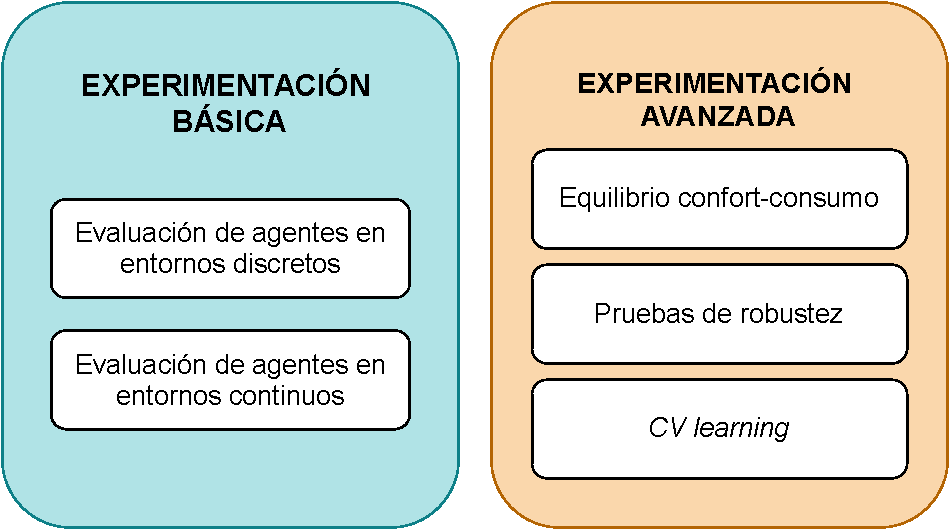
\includegraphics[width=\textwidth]{imagenes/metodologia.pdf}
    \caption{Experimentos realizados empleando Energym}
    \label{fig:metodologia}
\end{figure}

\section{Entorno de simulación}

La experimentación se desarrollará sobre una serie de entornos de simulación, compuestos por un modelo de edificio, diferentes tipos de clima y un conjunto de variables de entrada y salida ofrecidas por el simulador.

\subsection{Edificio}

El modelo de edificio empleado fue \texttt{5ZoneAutoDXVAV}: un edificio de 5 zonas (4 exteriores y 1 interior) climatizadas por medio de un sistema de aire acondicionado de tipo DX (\textit{Direct Expansion Air Conditioning Unit)}\footnote{Para más información sobre este tipo de sistemas, véase: \url{https://www.airconditioning-systems.com/direct-expansion-system.html}}. 

Se trata de un modelo incluido en el repositorio de modelos de ejemplo de EnergyPlus\footnote{El listado completo puede consultarse en: \url{https://github.com/NREL/EnergyPlus/tree/v8.6.0/testfiles}.} y previamente empleado en la literatura relacionada \cite{zhang2018practical}. La experimentación realizada se correspondió con el control de temperatura de una de las estancias.

\subsection{Climas}

Para llevar a cabo la simulación energética de un edificio, es necesario conocer las condiciones climáticas que lo atañen. Dichas condiciones pueden resumirse en un conjunto de datos correspondientes a un período de tiempo y lugar determinados, para posteriormente emplearse en la recreación de ese mismo contexto. 

La clasificación ofrecida por el DOE (Departamento de Energía de Estados Unidos) diferencia entre 19 tipos de clima\footnote{Dicha clasificación puede consultarse en el siguiente enlace: \url{https://www.energycodes.gov/development/commercial/prototype_models}}, desde extremadamente húmedos y cálidos, hasta árticos. Actualmente se encuentran disponibles numerosos repositorios con modelos abiertos de clima destinados a la simulación energética de edificios, como \href{http://climate.onebuilding.org/}{\textit{Climate.OneBuilding}}. En este caso, se utilizaron los tres modelos cuyas temperaturas se muestran en la Figura \ref{fig:weathers}, estos son:

\begin{itemize}
    \item \textbf{\href{https://www.energycodes.gov/sites/default/files/documents/USA_WA_Port.Angeles-William.R.Fairchild.Intl.AP.727885_TMY3.epw}{Clima frío}} (\texttt{cool marine, 5C}): correspondiente al aeropuerto \textit{William R. Fairchild International Airpor} (Washington) entre 1973 y 2005.
    \item \textbf{\href{https://www.energycodes.gov/sites/default/files/documents/USA_NY_New.York-John.F.Kennedy.Intl.AP.744860_TMY3.epw}{Clima templado}} (\texttt{mixed humid, 4A}): correspondiente al aeropuerto \textit{John F. Kennedy International Airport} (Nueva York) entre 1973 y 2005.
    \item \textbf{\href{https://www.energycodes.gov/sites/default/files/documents/USA_AZ_Tucson-Davis-Monthan.AFB.722745_TMY3.epw}{Clima cálido}} (\texttt{hot dry, 2B}): correspondiente a la base aérea \textit{Davis-Monthan Air Force} (Arizona) entre 1973 y 2005.
\end{itemize}

\begin{figure}
    \centering
    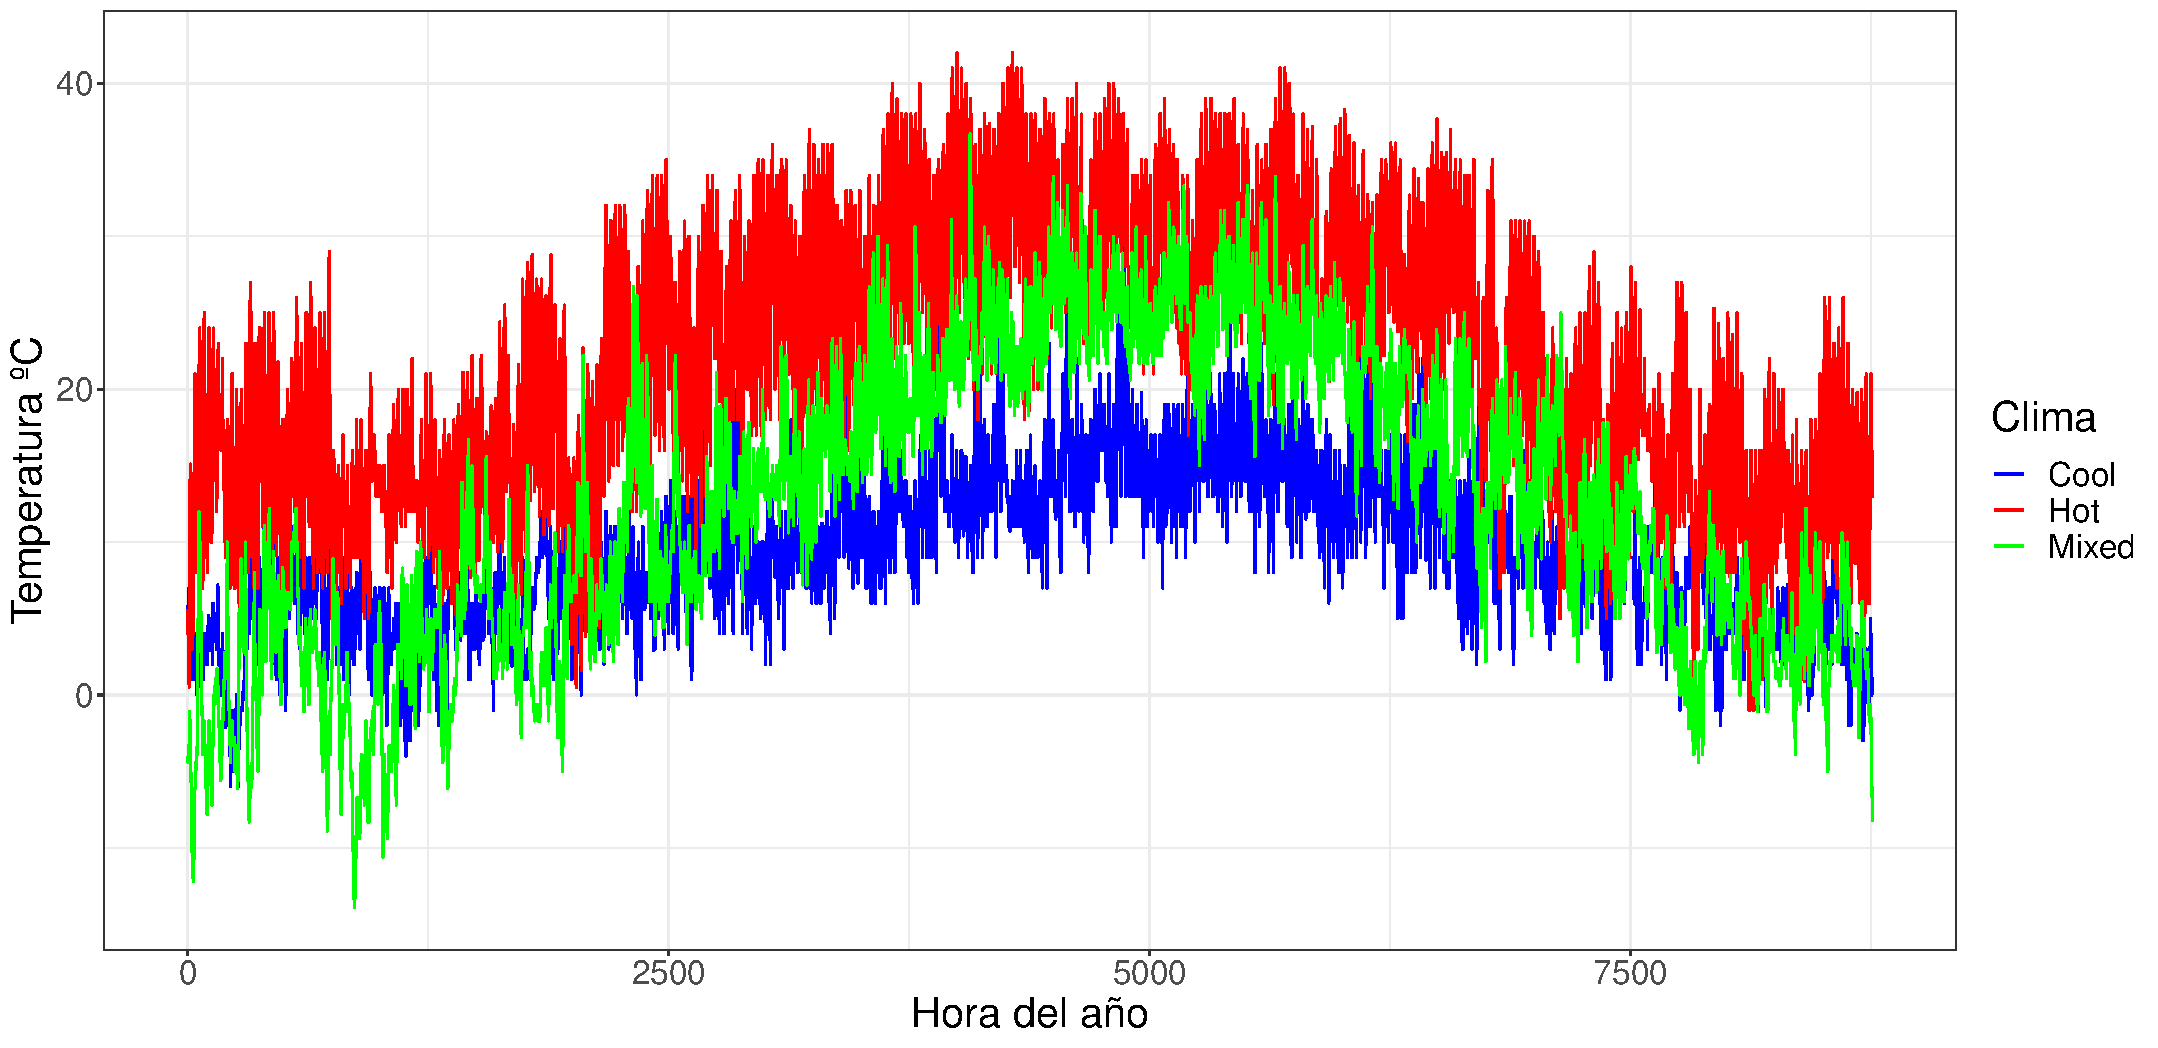
\includegraphics[width=\textwidth]{imagenes/weathers.pdf}
    \caption{Temperaturas (\textit{drybulb}) correspondientes a cada uno de los modelos de clima empleados en la experimentación (se representan los valores medios en cada una de las horas del año)}
    \label{fig:weathers}
\end{figure}

Tal y como se comentó en la sección \ref{sec:entornos}, la inclusión de ruido en estos conjuntos de datos favorece el entrenamiento y permite a los agentes contar con diferentes variaciones de un mismo clima episodio a episodio. Por tanto, los ficheros de clima empleados para realizar las simulaciones fueron una variante de los ya presentados, a los cuales se añadió cierta estocasticidad.

\subsection{Variables}
\label{sec:variables}

Toda simulación cuenta con una serie de variables de entrada (\textit{input variables}) y salida (\textit{output variables}). Mientras que las primeras son modificadas por el agente y tienen una influencia en el entorno, las segundas ofrecen información sobre su situación actual.

En el marco de esta experimentación, un total de 19 variables componen la observación que un agente recibe del entorno\footnote{Véase: \url{https://energym.readthedocs.io/en/latest/pages/environments.html\#observation-action-spaces}}. Estas son:

\begin{itemize}
    \item\textbf{Temperatura seca del aire en el exterior} (\textit{Site Outdoor Air Drybulb Temperature}).
    \item \textbf{Humedad relativa del aire en el exterior} (\textit{Site Outdoor Air Relative Humidity}).
    \item \textbf{Velocidad del viento} (\textit{Site Wind Speed}).
    \item \textbf{Dirección del viento} (\textit{Site Wind Direction}).
    \item \textbf{Radiación solar difusa por área} (\textit{Site Diffuse Solar Radiation Rate per Area }).
    \item \textbf{Radiación solar directa por área} (\textit{Site Diffuse Solar Radiation Rate per Area}).
    \item \textbf{Temperatura de consigna} (\textit{setpoint}) actual para \textbf{calefacción} (\textit{Zone Thermostat Heating Setpoint Temperature}).
    \item \textbf{Temperatura de consigna} (\textit{setpoint}) actual para \textbf{refrigeración} (\textit{Zone Thermostat Cooling Setpoint Temperature}).
    \item \textbf{Temperatura del aire} (\textit{Zone Air Temperature}).
    \item \textbf{Confort de acuerdo a la temperatura radiante media} (\textit{Zone Thermal Comfort Mean Radiant Temperature}).
    \item \textbf{Humedad relativa del aire} (\textit{Zone Air Relative Humidity}).
    \item \textbf{Confort termal de acuerdo al ropaje} (\textit{Zone Thermal Comfort Clothing Value}).
    \item \textbf{Confort termal de acuerdo al modelo Fanger PPD} (\textit{Zone Thermal Comfort Fanger Model PPD}).
    \item \textbf{Número de ocupantes} (\textit{Zone People Occupant Count}).
    \item \textbf{Temperatura del aire de acuerdo al modelo Fanger} (\textit{People Air Temperature}).
    \item \textbf{Demanda energética de dispositivos HVAC} (\textit{Facility Total HVAC Electric Demand Power}).
    \item \textbf{Día} (\textit{Current Day}).
    \item \textbf{Mes} (\textit{Current Month}).
    \item \textbf{Hora} (\textit{Current Hour}).
\end{itemize}

Por otro lado, las variables de entrada modificadas por el agente se corresponden con las ya descritas en la sección \ref{sec:entornos}:

\begin{itemize}
    \item \textbf{\textit{Setpoint} de calefacción }(\textit{Heating Setpoint}).
    \item \textbf{\textit{Setpoint} de refrigeración} (\textit{Cooling Setpoint}).
\end{itemize}

De esta forma, todo agente recibirá como observación el conjunto de variables inicialmente descrito, y actuará en consecuencia modificando los \textit{setpoints} de acuerdo a sus objetivos de consumo y confort. 

\subsection{Métricas de evaluación}
\label{sec:metricas-evaluacion}

Finalmente, evaluaremos el desempeño de los agentes centrándonos en un conjunto métricas derivadas de las variables de salida previamente descritas. Estas métricas, ejemplificadas en la Figura \ref{fig:DDPG-results}, son las siguientes:

\begin{figure}
    \centering
    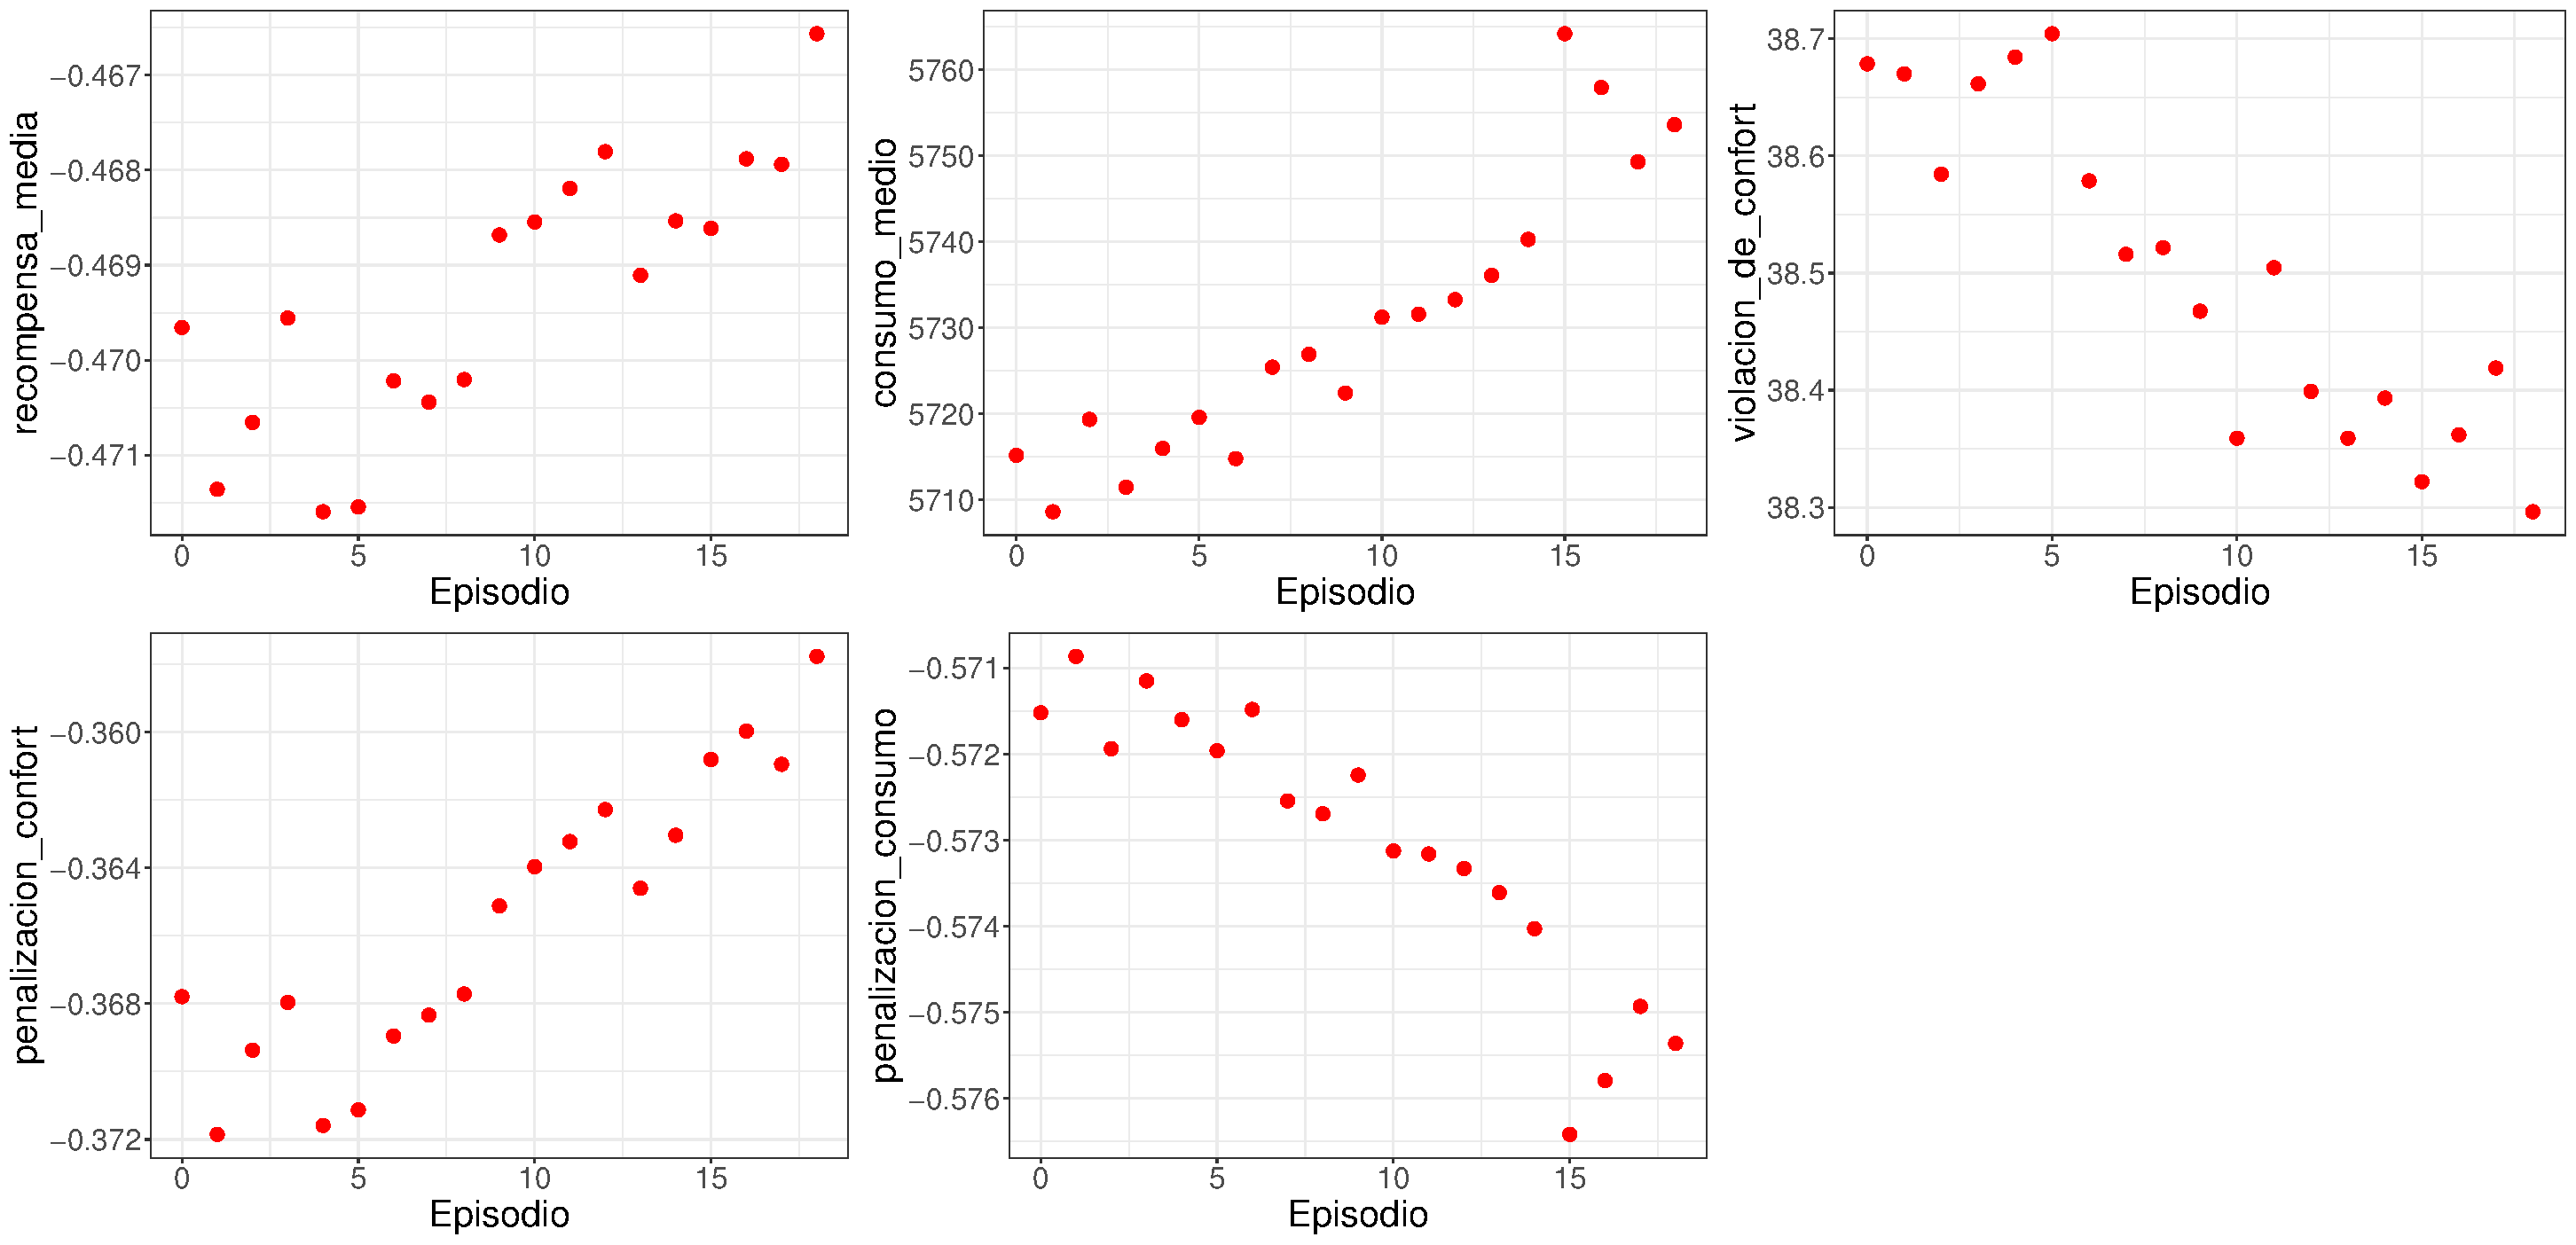
\includegraphics[width=\textwidth]{imagenes/ddpg-cont-mixed-fixed.pdf}
    \caption{Ejemplo de las métricas evaluadas durante la validación de DDPG en el entorno \textit{continuous-stochastic-mixed}}
    \label{fig:DDPG-results}
\end{figure}

\begin{itemize}
    \item \textbf{Recompensa media}: nos indica cómo de bien o mal el agente está garantizando un control eficiente que respete el confort de los ocupantes del edificio y reduzca el consumo.
    
    Recordemos que, tal y como se introdujo en la sección \ref{sec:formulacion}, la función de recompensa empleada por los agentes es la siguiente:
    
    \begin{equation}
        \label{eq:reward-simple}
        r(S_t, A_t) = - w_t \cdot \lambda_c \cdot Confort - (1-w_t) \cdot \lambda_e \cdot Consumo
    \end{equation}
    
     Al estar expresada en términos negativos, buscamos que se mantenga lo más próxima a $0$ posible, o lo que es lo mismo: maximizarla. Así, el cálculo de la recompensa media será igual al promedio de las recompensas medias obtenidas por los agentes en cada episodio.
    
    \item \textbf{Consumo medio}: indica el consumo energético medio a lo largo de la simulación, correspondiente a la variable de salida \textit{Facility Total HVAC Electric Demand Power}. 
    
    Aunque escapa del ámbito de este trabajo profundizar en aspectos referentes al consumo energético, penalización energética, etc., se dota de herramientas a aquellos expertos que deseen hacer un análisis más exhaustivo de estas métricas.
    
    \item \textbf{Violación de confort}: mide el porcentaje de tiempo de un episodio en el que no se ha respetado el intervalo de temperaturas de confort establecidas por el usuario.
    
    \item \textbf{Penalizaciones por confort y consumo} indican el valor medio para cada una de las partes de la recompensa episodio a episodio.
    
    Partiendo de la ecuación \ref{eq:reward-simple}, denominamos ``penalización por consumo'' a: $(1-w_t) \cdot \lambda_e \cdot Consumo$, mientras que $w_t \cdot \lambda_c \cdot Confort$ es la ``penalización por confort''.
\end{itemize}

Una vez presentadas estas métricas, profundizaremos en su análisis para cada uno de los agentes en la sección \ref{sec:results}.

\section{Entrenamiento y evaluación de los agentes}
\label{sec:evaluacion-agentes}

Una vez definidas las condiciones de nuestro experimento, en las siguientes subsecciones evaluaremos los resultados obtenidos tras el entrenamiento y evaluación de los agentes en los entornos discretos y continuos.

El \textit{hardware} empleado para entrenar a los agentes consistió en un equipo \textit{HP Pavilion x360 convertible 14-cd0xxx} equipado con:

\begin{itemize}
    \item Procesador \textit{Intel Core i7-8550U CPU @ 1.80GHz 1.99GHz} de 64 bits.
    \item 12 GB de RAM.
    \item Tarjeta gráfica integrada \textit{Intel UHD Graphics 620}.
    \item Tarjeta gráfica externa \textit{NVIDIA GeForce MX130}.
\end{itemize}

\FloatBarrier
\subsection{Espacio de acciones discreto}

Los algoritmos empleados en los entornos discretos fueron \textbf{DQN}, \textbf{A2C} y \textbf{PPO}. Su entrenamiento fue monitorizado mediante TensorBoard (Figura \ref{fig:train-disc}) y se consideró la siguiente configuración:

\begin{itemize}
    \item Número de episodios de entrenamiento: 20.
    \item Evaluaciones periódicas durante el entrenamiento cada 5 episodios.
    \item Episodios empleados para evaluar durante el entrenamiento: 2.
    \item Hiperparámetros por defecto para todos los algoritmos.
    \item Misma ponderación para confort y consumo ($w_t = 0.5$).
    \item Mismo entorno para entrenamiento y evaluación, con variaciones en el clima episodio a episodio en ambos casos.
\end{itemize}

\begin{figure}
    \centering
    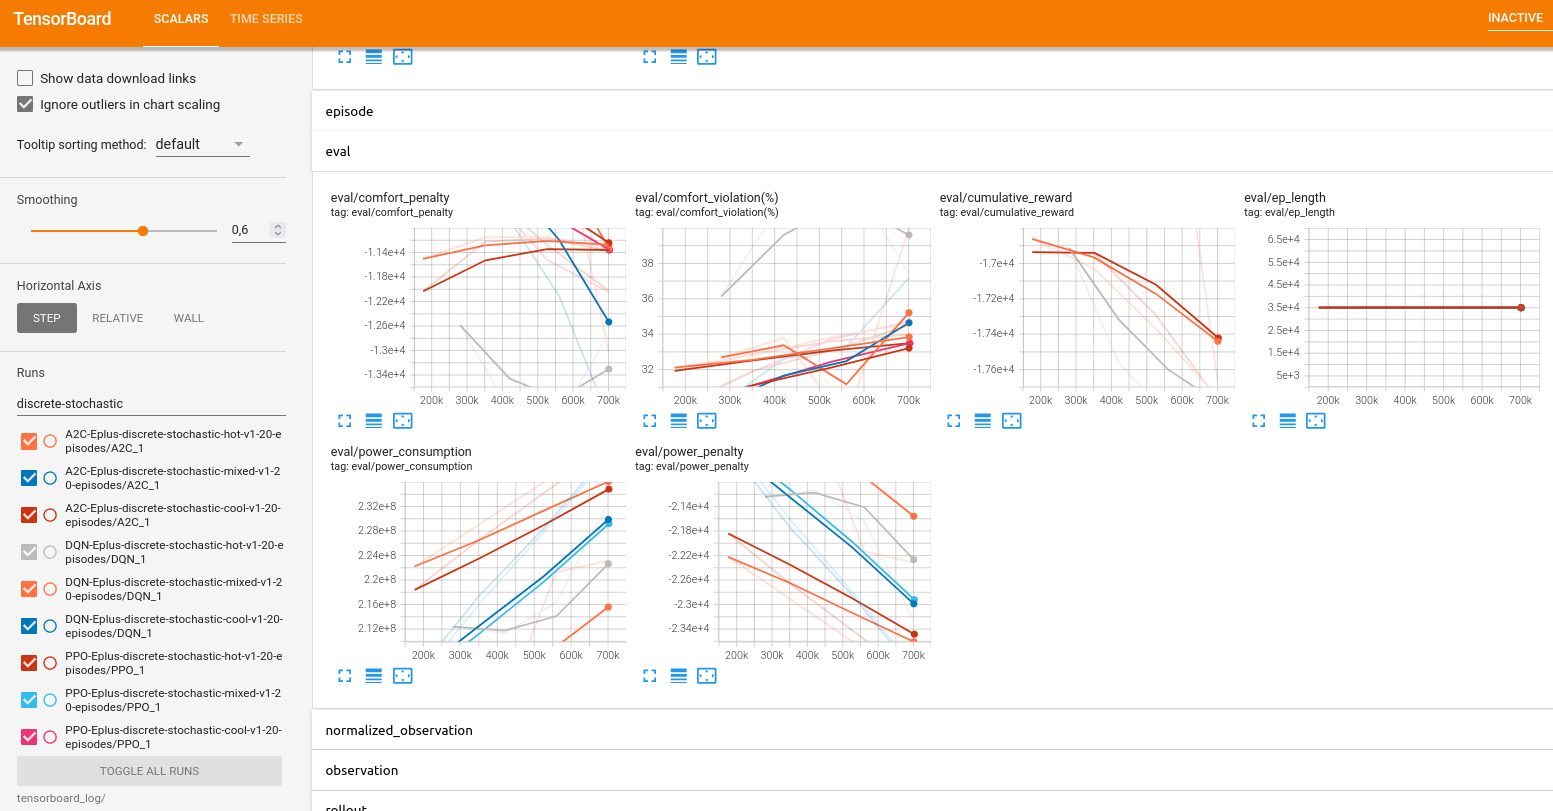
\includegraphics[width=\textwidth]{imagenes/entrenamiento-discretos.png}
    \caption{Proceso de entrenamiento de los entornos discretos monitorizado mediante TensorBoard}
    \label{fig:train-disc}
\end{figure}

Atendiendo a la convergencia de los diferentes modelos, A2C logró converger más rápidamente que el resto, seguido por DQN y PPO. Un ejemplo ilustrativo de dicha convergencia es el que se muestra en la Figura \ref{fig:train-disc-confort}, donde se compara la evolución de la violación de confort para A2C y DQN. En la figura puede verse cómo, a medida que los agentes son entrenados, estos perfeccionan sus políticas, lo que deriva en una reducción de las violaciones de confort y, junto a la reducción del consumo, en una mejora progresiva de las recompensas obtenidas.

\begin{figure}
    \centering
    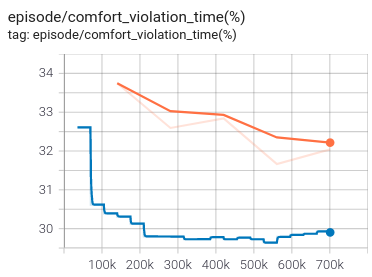
\includegraphics[width=0.7\textwidth]{imagenes/train-disc-violacion-confort.png}
    \caption{Monitorización mediante TensorBoard de la evolución y convergencia de la violación de confort para A2C (azul) y DQN (naranja) en el entorno \textit{discrete-mixed}}
    \label{fig:train-disc-confort}
\end{figure}

Una vez entrenados, se procedió a la validación del mejor modelo obtenido para cada algoritmo de DRL, así como de un agente basado en reglas (RBC) de cara a poder comparar. Dicha validación consistió en la ejecución de cada modelo durante un total de 20 episodios, lo que sirvió para comprobar la generalización y adaptabilidad de los agentes a medida que el ruido sobre el clima se iba acumulando\footnote{Evaluaciones de tal longitud no son comunes en la literatura, siendo 1 ó 2 episodios los empleados normalmente para validar un agente ya entrenado. No obstante, como se ha indicado, una validación mucho más prologada permite conocer la capacidad de generalización de los agentes a medida que las condiciones climáticas se vuelven más extremas.}.

Como se detallará en la sección \ref{sec:results}, se observó un rendimiento significativamente bajo (en comparación con el RBC) en prácticamente la totalidad de los casos, pudiendo deberse este bajo rendimiento a la dependencia entre \textit{setpoints} fríos y calientes y al uso un espacio de acciones quizá demasiado limitado. Esto no fue un problema para los agentes en entornos continuos, donde cada \textit{setpoint} pudo tomar valores de forma independiente.

\FloatBarrier
\subsection{Espacio de acciones continuo}

En el caso de los entornos con espacios de acciones continuos, los algoritmos empleados fueron \textbf{DDPG}, \textbf{PPO}, \textbf{A2C} y \textbf{SAC}. Por otro lado, las condiciones de entrenamiento (ver Figuras \ref{fig:train-cont} y \ref{fig:train-cont-confort}) fueron las mismas que las de los algoritmos en entornos discretos.

\begin{figure}
    \centering
    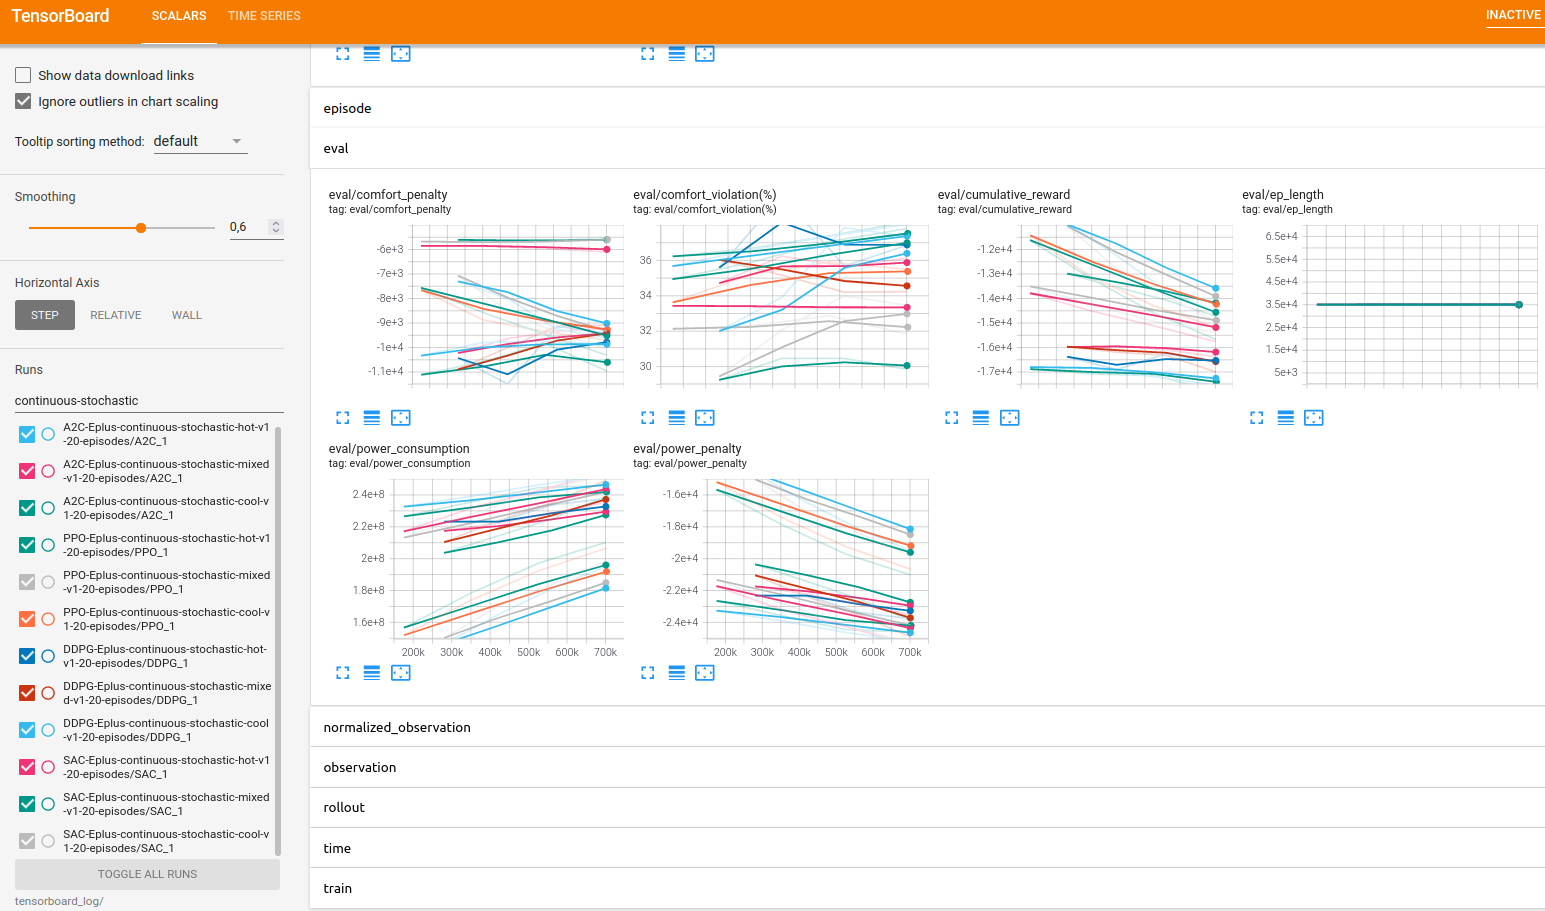
\includegraphics[width=\textwidth]{imagenes/entrenamiento-continuos.png}
    \caption{Proceso de entrenamiento de los entornos continuos monitorizado mediante TensorBoard}
    \label{fig:train-cont}
\end{figure}

\begin{figure}
    \centering
    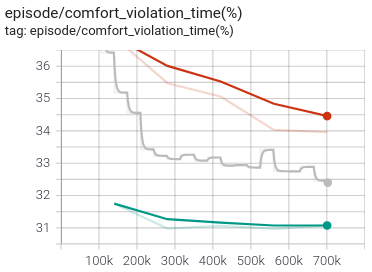
\includegraphics[width=0.7\textwidth]{imagenes/train-cont-confort-violation.png}
    \caption{Monitorización mediante TensorBoard de la evolución y convergencia de la violación de confort para DDPG (rojo), PPO (gris) y SAC (verde) en el entorno \textit{continous-mixed}}
    \label{fig:train-cont-confort}
\end{figure}

Aunque más adelante profundizaremos en los resultados obtenidos, inicialmente se comprobó que:

\begin{itemize}
    \item A2C presenta un comportamiento prácticamente similar a RBC en todos los escenarios.
    \item PPO se comporta de forma similar a A2C y RBC en el entorno templado y ofrece peores resultados para los climas cálido y frío.
    \item DDPG obtiene peores resultados con respecto al resto de algoritmos en entornos templados, pero destaca junto a SAC en los entornos cálido y frío.
    \item SAC presenta los mejores resultados, con un rendimiento generalmente superior al resto (especialmente en el entorno templado), aunque similar al de DDPG en los climas cálido y frío.
\end{itemize}

Un aspecto importante a considerar es cómo la convergencia de los agentes en entornos continuos fue considerablemente más lenta que la de los basados en espacios de acciones discretos. Por lo general, se requiere de un mayor tiempo de entrenamiento para que los algoritmos en entornos continuos alcancen sus mejores resultados.

Finalmente, tanto en los entornos discretos como continuos se observó que un mayor tiempo de entrenamiento supone, a largo plazo, un rendimiento mucho mejor. No obstante, dados los altos requisitos computacionales que supone dicho entrenamiento (con tiempos de entrenamiento para 20 episodios de hasta 3 horas en entornos discretos y 9 horas en los continuos), centraremos nuestra atención en ilustrar los resultados obtenidos para esta prueba limitada a 20 episodios.

\FloatBarrier
\subsection{Resultados}
\label{sec:results}

El entrenamiento de los diferentes agentes, tanto en entornos discretos como continuos, dio lugar a una gran cantidad de datos y gráficas correspondientes a las variables monitorizadas por TensorBoard. Como escapa del ámbito de este trabajo realizar un análisis en profundidad de cada métrica y algoritmo, nos centraremos en estudiar el rendimiento de los agentes desde la perspectiva de las métricas de evaluación previamente presentadas en la sección \ref{sec:metricas-evaluacion}: \textbf{recompensa} (recompensa media), \textbf{consumo} (consumo medio y penalización por consumo) y \textbf{confort} (violación de confort y penalización por confort). 

Así, basándonos en los resultados obtenidos en la validación de los agentes, en la Tabla \ref{tb:best-models} se muestra una perspectiva general de los mejores algoritmos para cada entorno, desde el punto de vista de estas métricas de evaluación.

\begin{table}
    \centering
    \caption{Mejores agentes para diferentes entornos y métricas}
    \label{tb:best-models}
    \resizebox{\textwidth}{!}{%
    \begin{tabular}{cccc}
    \textbf{Entorno} & \textbf{Recompensa} & \textbf{Consumo} & \textbf{Confort} \\ \hline
    \textbf{Disc. hot} & RBC/A2C & DQN & RBC/A2C \\ \hline
    \textbf{Disc. mixed} & RBC & DQN & RBC/A2C \\ \hline
    \textbf{Disc. cool} & RBC/A2C & PPO & RBC/A2C \\ \hline
    \textbf{Cont. hot} & DDPG/SAC & SAC & DDPG \\ \hline
    \textbf{Cont. mixed} & DDPG/SAC & DDPG & SAC \\ \hline
    \textbf{Cont. cool} & SAC & SAC & SAC\\ \hline
    \end{tabular}%
    }
\end{table}

Como se mencionó anteriormente, el rendimiento de los algoritmos en espacios de acciones discretos fue significativamente peor que en los continuos, acercándose al controlador basado en reglas pero sin llegar a superarlo en la mayoría de los casos. Por otro lado, también se enfatizó en el hecho de que los agentes en entornos continuos requieren de un mayor número de episodios para converger en su entrenamiento, al tratarse de espacios de acciones mucho más complejos. Dicha complejidad se debe a que los \textit{setpoints} de calor y frío se ajustan con respecto a un intervalo de valores mucho mayor. De esta forma, estamos ante algoritmos más flexibles, donde no existe ninguna interdependencia entre ambos \textit{setpoints} que pueda afectar al rendimiento, como sí ocurre en los entornos discretos.

La solución al bajo rendimiento de los entornos discretos pasaría por ampliar el número de acciones disponibles, ofreciendo una posibilidad de mapeo mucho mayor, así como por la definición de espacios de acciones multidiscretos. Dichas propuestas están presentes en la sección \ref{sec:trabajo-futuro}, dedicada a aquellos trabajos futuros que puedan derivarse de este proyecto.

Hechas estas aclaraciones, pasemos a analizar cuantitativamente los resultados obtenidos en la \textbf{validación} de los agentes entrenados.

\subsubsection{Consumo energético}

Desde el punto de vista del consumo energético medio en los entornos discretos (Tabla \ref{tb:consumo-disc}), A2C ofreció unos resultados muy similares a los del RBC, sin ofrecer una mejora significativa en ninguno de los tres casos. Por otro lado, PPO logró una mejora del $2.87\%$ en el entorno frío, mientras que DQN redujo el consumo del RBC en los entornos cálido y templado, con disminuciones de consumo del $5.44\%$ y $6.12\%$, respectivamente. No obstante, debe destacarse que estas reducciones en el consumo repercutieron negativamente en el confort, como veremos a la hora de estudiar las recompensas obtenidas.

En el caso de los entornos continuos (Tabla \ref{tb:consumo-cont}), SAC y DDPG lograron mejorar los resultados del RBC con resultados bastante positivos: mientras que SAC logró un consumo un $7.67\%$ y $5.71\%$ inferior en los entornos \textit{hot} (Figura \ref{fig:consumo-cont-hot}) y \textit{mixed}, respectivamente, DDPG obtuvo el menor consumo en el entorno frío con una reducción del $7.45\%$.

\begin{table}
    \centering
    \caption{Consumo medio de los agentes entrenados en entornos discretos a lo largo de 20 episodios de validación}
    \label{tb:consumo-disc}
    \resizebox{0.8\textwidth}{!}{%
    \begin{tabular}{ccccccc}
     & \multicolumn{2}{c}{\textbf{HOT}} & \multicolumn{2}{c}{\textbf{COOL}} & \multicolumn{2}{c}{\textbf{MIXED}} \\ \hline
     & \textit{media} & \textit{desv} & \textit{media} & \textit{desv} & \textit{media} & \textit{desv} \\ \hline
    \textbf{RBC} & 6428 & 171 & 4421 & 507 & 5911 & 223 \\ \hline
    \textbf{A2C} & 6403 & 178 & 4426 & 524 & 5960 & 249 \\ \hline
    \textbf{PPO} & 6278 & 139 & \textbf{4294} & 490 & 5800 & 229 \\ \hline
    \textbf{DQN} & \textbf{6078} & 149 & 4369 & 505 & \textbf{5549} & 238 \\ \hline
    \end{tabular}%
    }
\end{table}

\begin{table}
    \centering
    \caption{Consumo medio de los agentes entrenados en entornos continuos a lo largo de 20 episodios de validación}
    \label{tb:consumo-cont}
    \resizebox{0.8\textwidth}{!}{%
    \begin{tabular}{ccccccc}
     & \multicolumn{2}{c}{\textbf{HOT}} & \multicolumn{2}{c}{\textbf{COOL}} & \multicolumn{2}{c}{\textbf{MIXED}} \\ \hline
     & \textit{media} & \textit{desv} & \textit{media} & \textit{desv} & \textit{media} & \textit{desv} \\ \hline
    \textbf{RBC} & 6674 & 164 & 4612 & 486 & 6220 & 249 \\ \hline
    \textbf{A2C} & 6664 & 160 & 4630 & 522 & 6223 & 267 \\ \hline
    \textbf{PPO} & 6326 & 122 & 4462 & 486 & 6146 & 260 \\ \hline
    \textbf{DDPG} & 6371 & 132 & \textbf{4268} & 465 & 6119 & 234 \\ \hline
    \textbf{SAC} & \textbf{6162} & 122 & 4359 & 514 & \textbf{5865} & 239 \\ \hline
    \end{tabular}%
    }
\end{table}

\begin{figure}
    \centering
    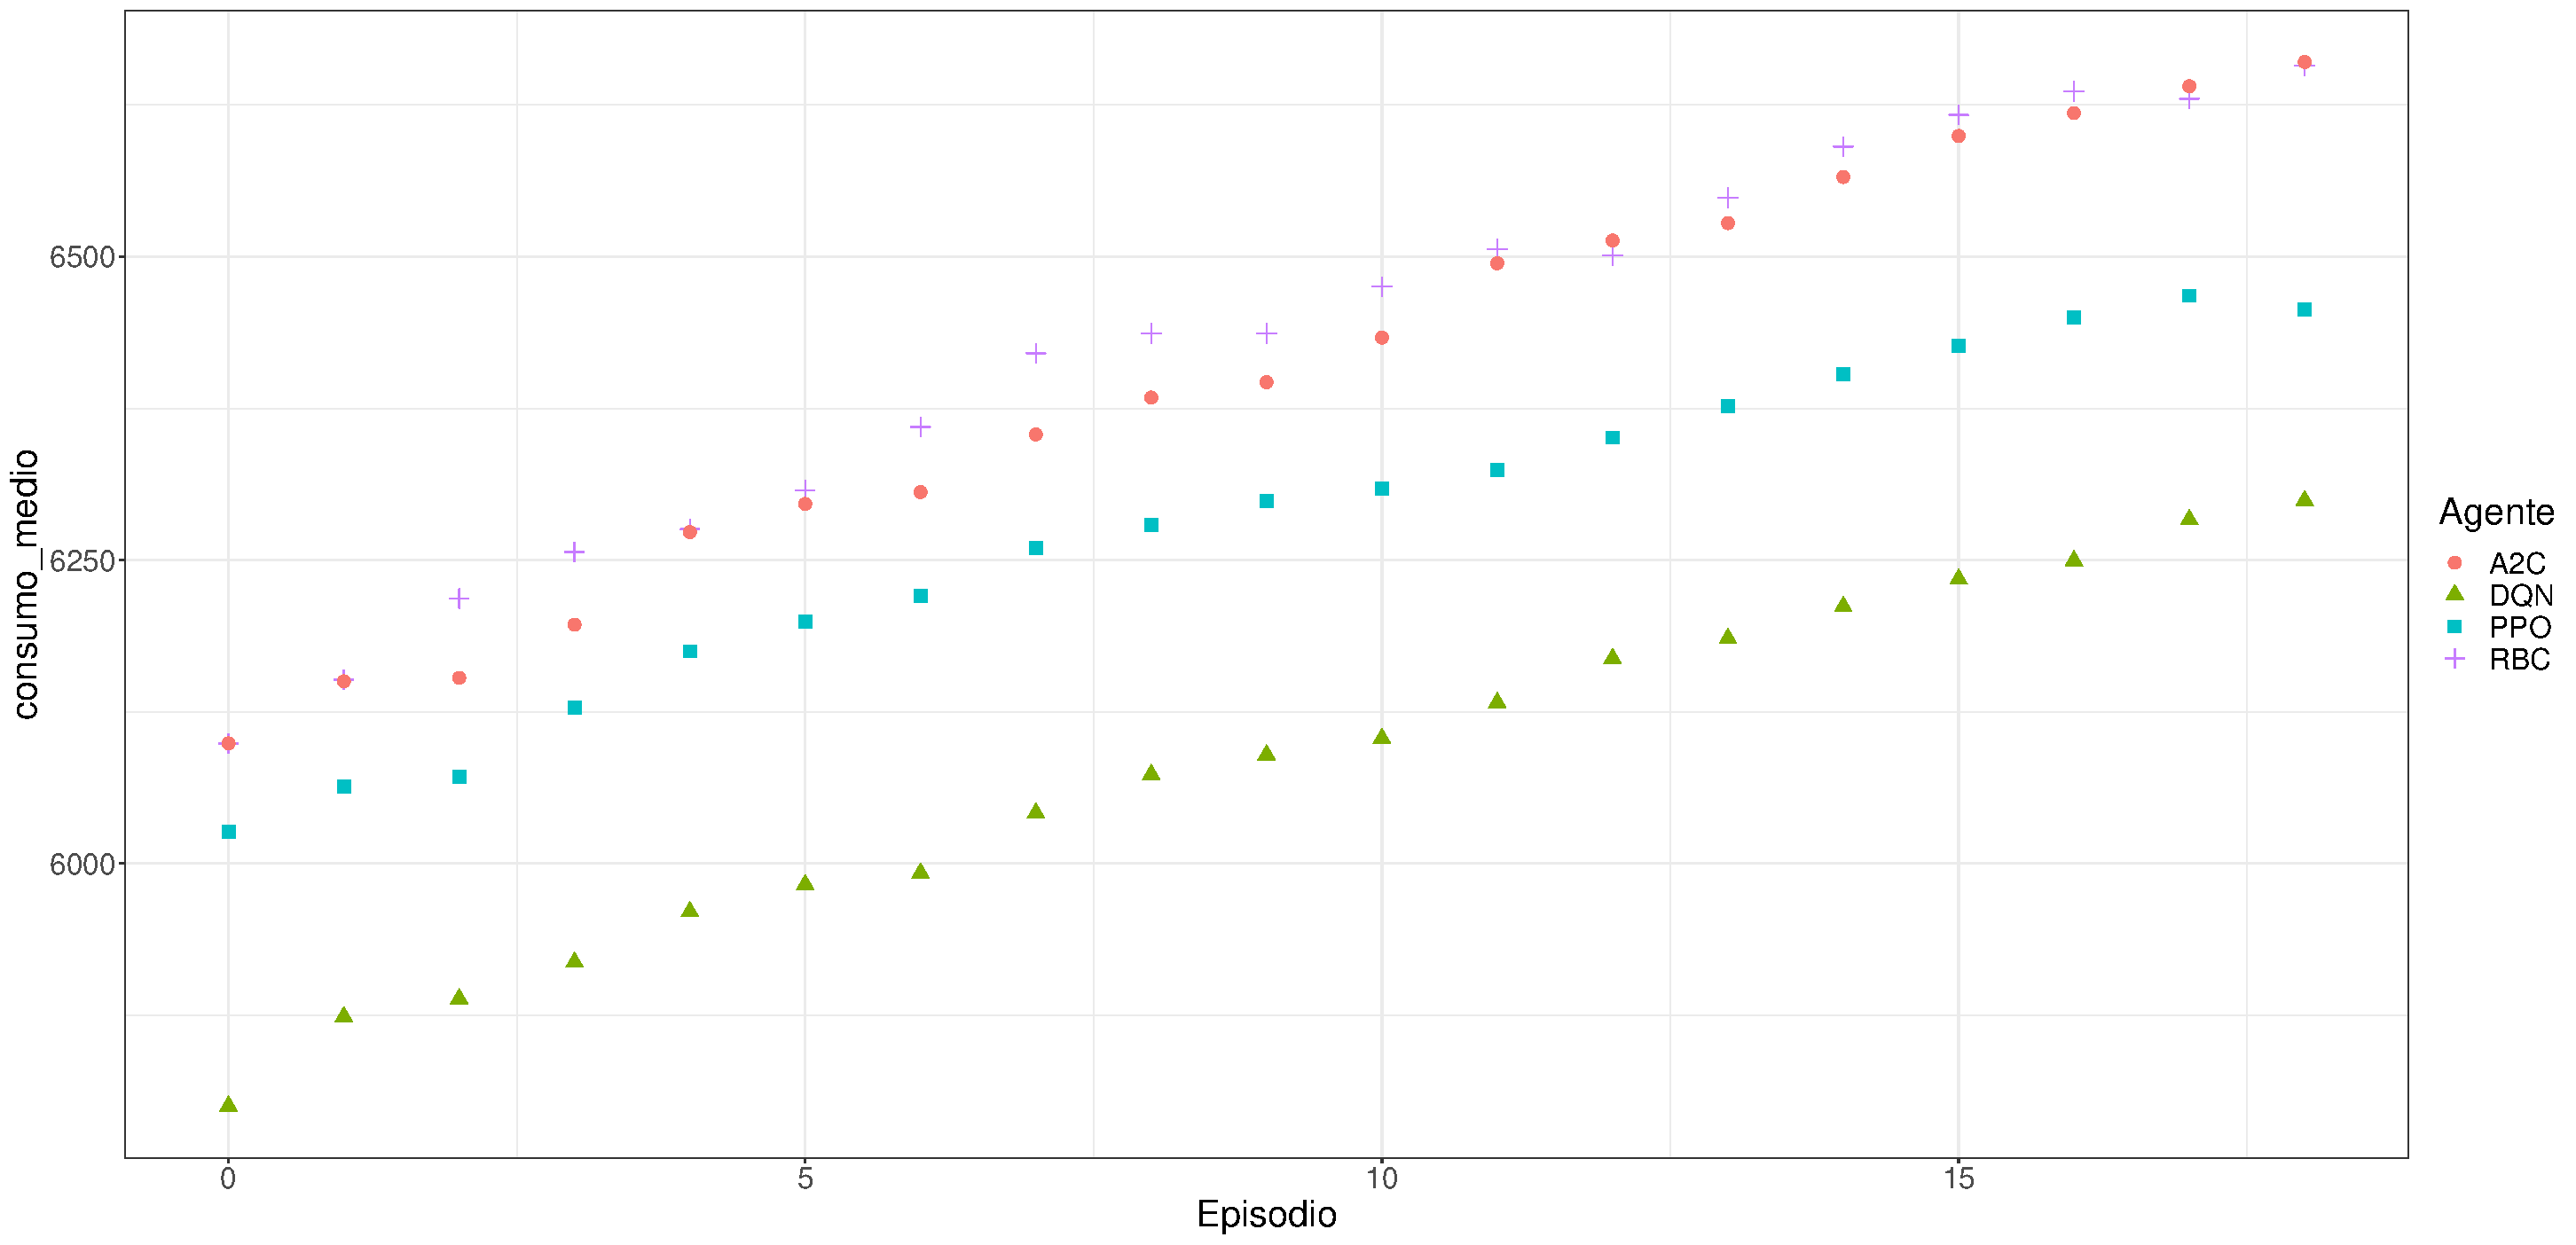
\includegraphics[width=\textwidth]{imagenes/consumo-disc-hot.pdf}
    \caption{Ejemplo del consumo medio obtenido en la validación de los agentes entrenados en el entorno \textit{discrete-stochastic-hot}}
    \label{fig:consumo-disc-hot}
\end{figure}

\begin{figure}
    \centering
    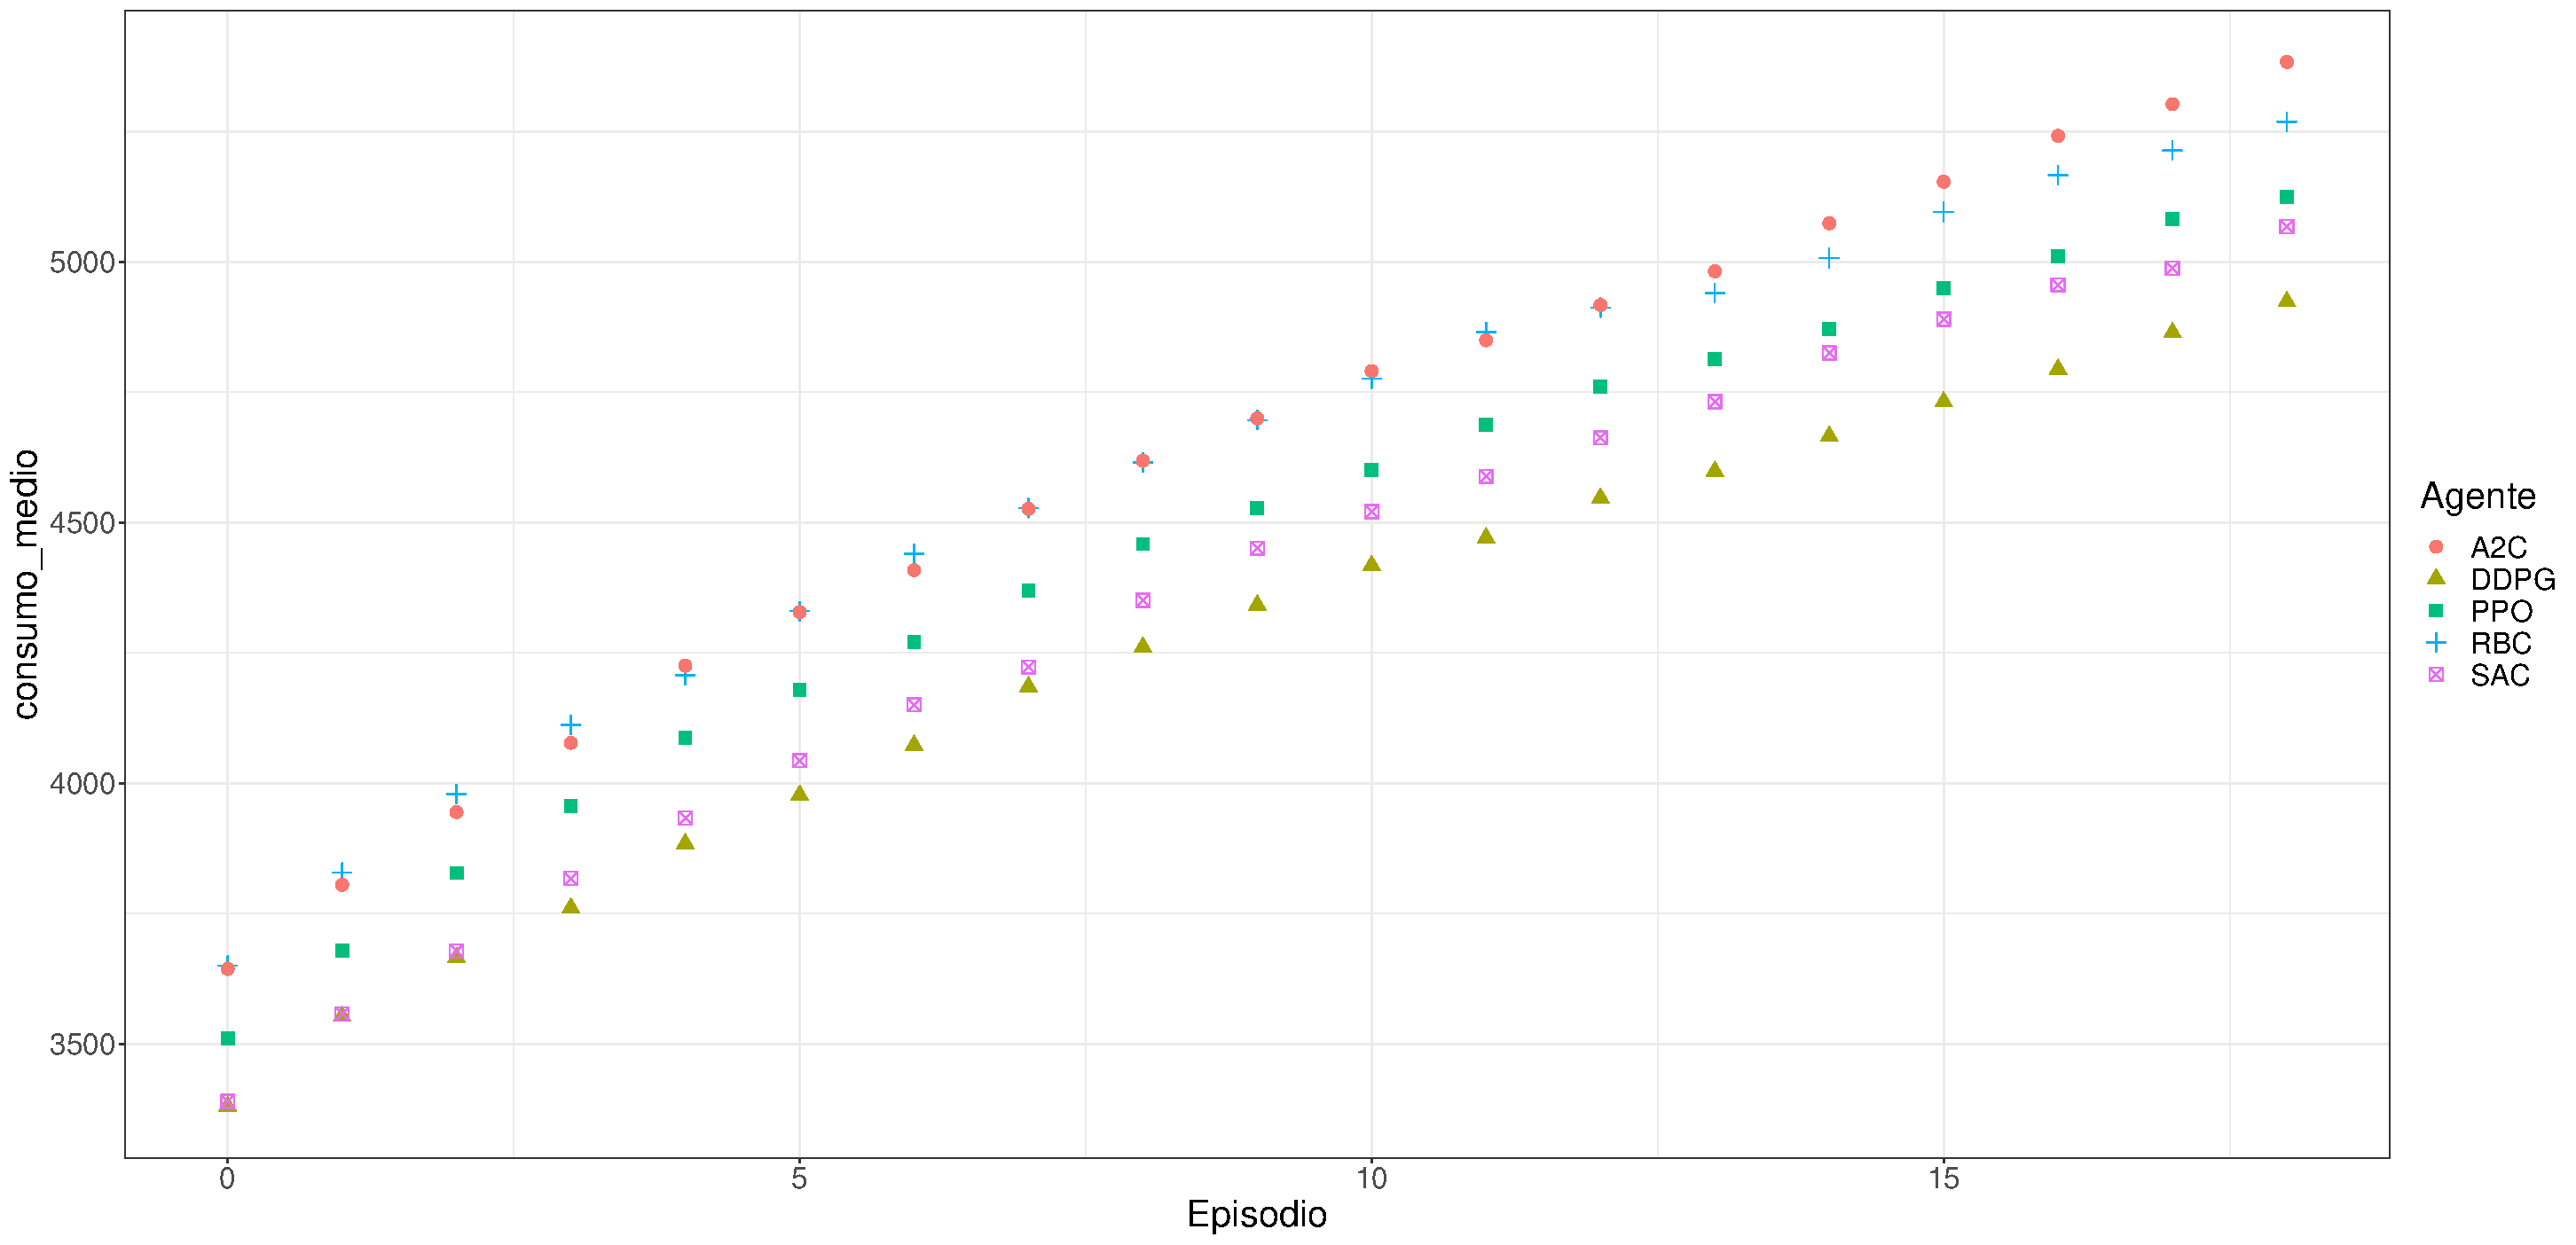
\includegraphics[width=\textwidth]{imagenes/consumo-cont-hot.pdf}
    \caption{Ejemplo del consumo medio obtenido en la validación de los agentes entrenados en el entorno \textit{continuous-stochastic-hot}}
    \label{fig:consumo-cont-hot}
\end{figure}

Finalmente, nótese cómo, tanto en los entornos discretos como continuos, el consumo medio representado en las Figuras \ref{fig:consumo-disc-hot} y \ref{fig:consumo-cont-hot} es creciente debido a la acumulación de ruido en el clima a lo largo del tiempo, lo que dificulta la optimización del consumo energético.

\subsubsection{Confort}

Tomando como referencia el porcentaje de tiempo bajo violación de confort en los entornos discretos, RBC ($32.5\%$) y A2C ($32.6\%$) ofrecieron un desempeño similar para el clima cálido. En el clima templado, los porcentajes fueron del $29.9\%$ y $30\%$, respectivamente, mientras que en el frío, RBC logró un $30.4\%$, A2C un $30.2\%$ y DQN un $31.5\%$. Así, atendiendo a los resultados de la Tabla \ref{tb:confort-disc}, ningún algoritmo de DRL logró mejorar significativamente los resultados del RBC.

Desde la perspectiva de los entornos continuos, se lograron resultados más positivos (ver Tabla \ref{tb:confort-cont}). Frente al bajo rendimiento de A2C y PPO, DDPG logró reducir en un $2.6\%$ la violación de confort con respecto al RBC en clima cálido, mientras que SAC consiguió reducciones del $4.1\%$ y $0.9\%$ en los entornos frío y templado (Figura \ref{fig:confort-cont-mixed}), respectivamente. Aunque no se trata de grandes reducciones en la violación de confort, en la siguiente sección veremos cómo, en combinación con la reducción del consumo, estas se tradujeron en un considerable aumento de las recompensas obtenidas.

\begin{table}
    \centering
    \caption{Violación de confort media de los agentes entrenados en entornos discretos a lo largo de 20 episodios de validación}
    \label{tb:confort-disc}
    \resizebox{0.8\textwidth}{!}{%
    \begin{tabular}{ccccccc}
     & \multicolumn{2}{c}{\textbf{HOT}} & \multicolumn{2}{c}{\textbf{COOL}} & \multicolumn{2}{c}{\textbf{MIXED}} \\ \hline
     & \textit{media} & \textit{desv} & \textit{media} & \textit{desv} & \textit{media} & \textit{desv} \\ \hline
    \textbf{RBC} & \textbf{32.5} & .942 & 30.4 & 1.5 & \textbf{29.9} & .296 \\ \hline
    \textbf{A2C} & 32.6 & .882 & \textbf{30.2} & 1.46 & 30 & .225 \\ \hline
    \textbf{PPO} & 33.9 & .778 & 35.4 & 1.48 & 32.1 & .313 \\ \hline
    \textbf{DQN} & 36.9 & 1.1 & 31.5 & 1.26 & 33.6 & .479 \\ \hline
    \end{tabular}%
    }
\end{table}

\begin{table}
    \centering
    \caption{Violación de confort media de los agentes entrenados en entornos continuos a lo largo de 20 episodios de validación}
    \label{tb:confort-cont}
    \resizebox{0.8\textwidth}{!}{%
    \begin{tabular}{ccccccc}
     & \multicolumn{2}{c}{\textbf{HOT}} & \multicolumn{2}{c}{\textbf{COOL}} & \multicolumn{2}{c}{\textbf{MIXED}} \\ \hline
     & \textit{media} & \textit{desv} & \textit{media} & \textit{desv} & \textit{media} & \textit{desv} \\ \hline
    \textbf{RBC} & 35.9 & .705 & 35.1 & .7 & 33.5 & .064 \\ \hline
    \textbf{A2C} & 36.1 & .675 & 35.1 & .701 & 33.6 & .038 \\ \hline
    \textbf{PPO} & 37.5 & .557 & 34.9 & .933 & 33.6 & .549 \\ \hline
    \textbf{DDPG} & \textbf{33.3} & .944 & 32.9 & 1.55 & 36 & 1.06 \\ \hline
    \textbf{SAC} & 35.7 & .843 & \textbf{31} & 1.29 & \textbf{32.6} & .336 \\ \hline
    \end{tabular}%
    }
\end{table}

\begin{figure}
    \centering
    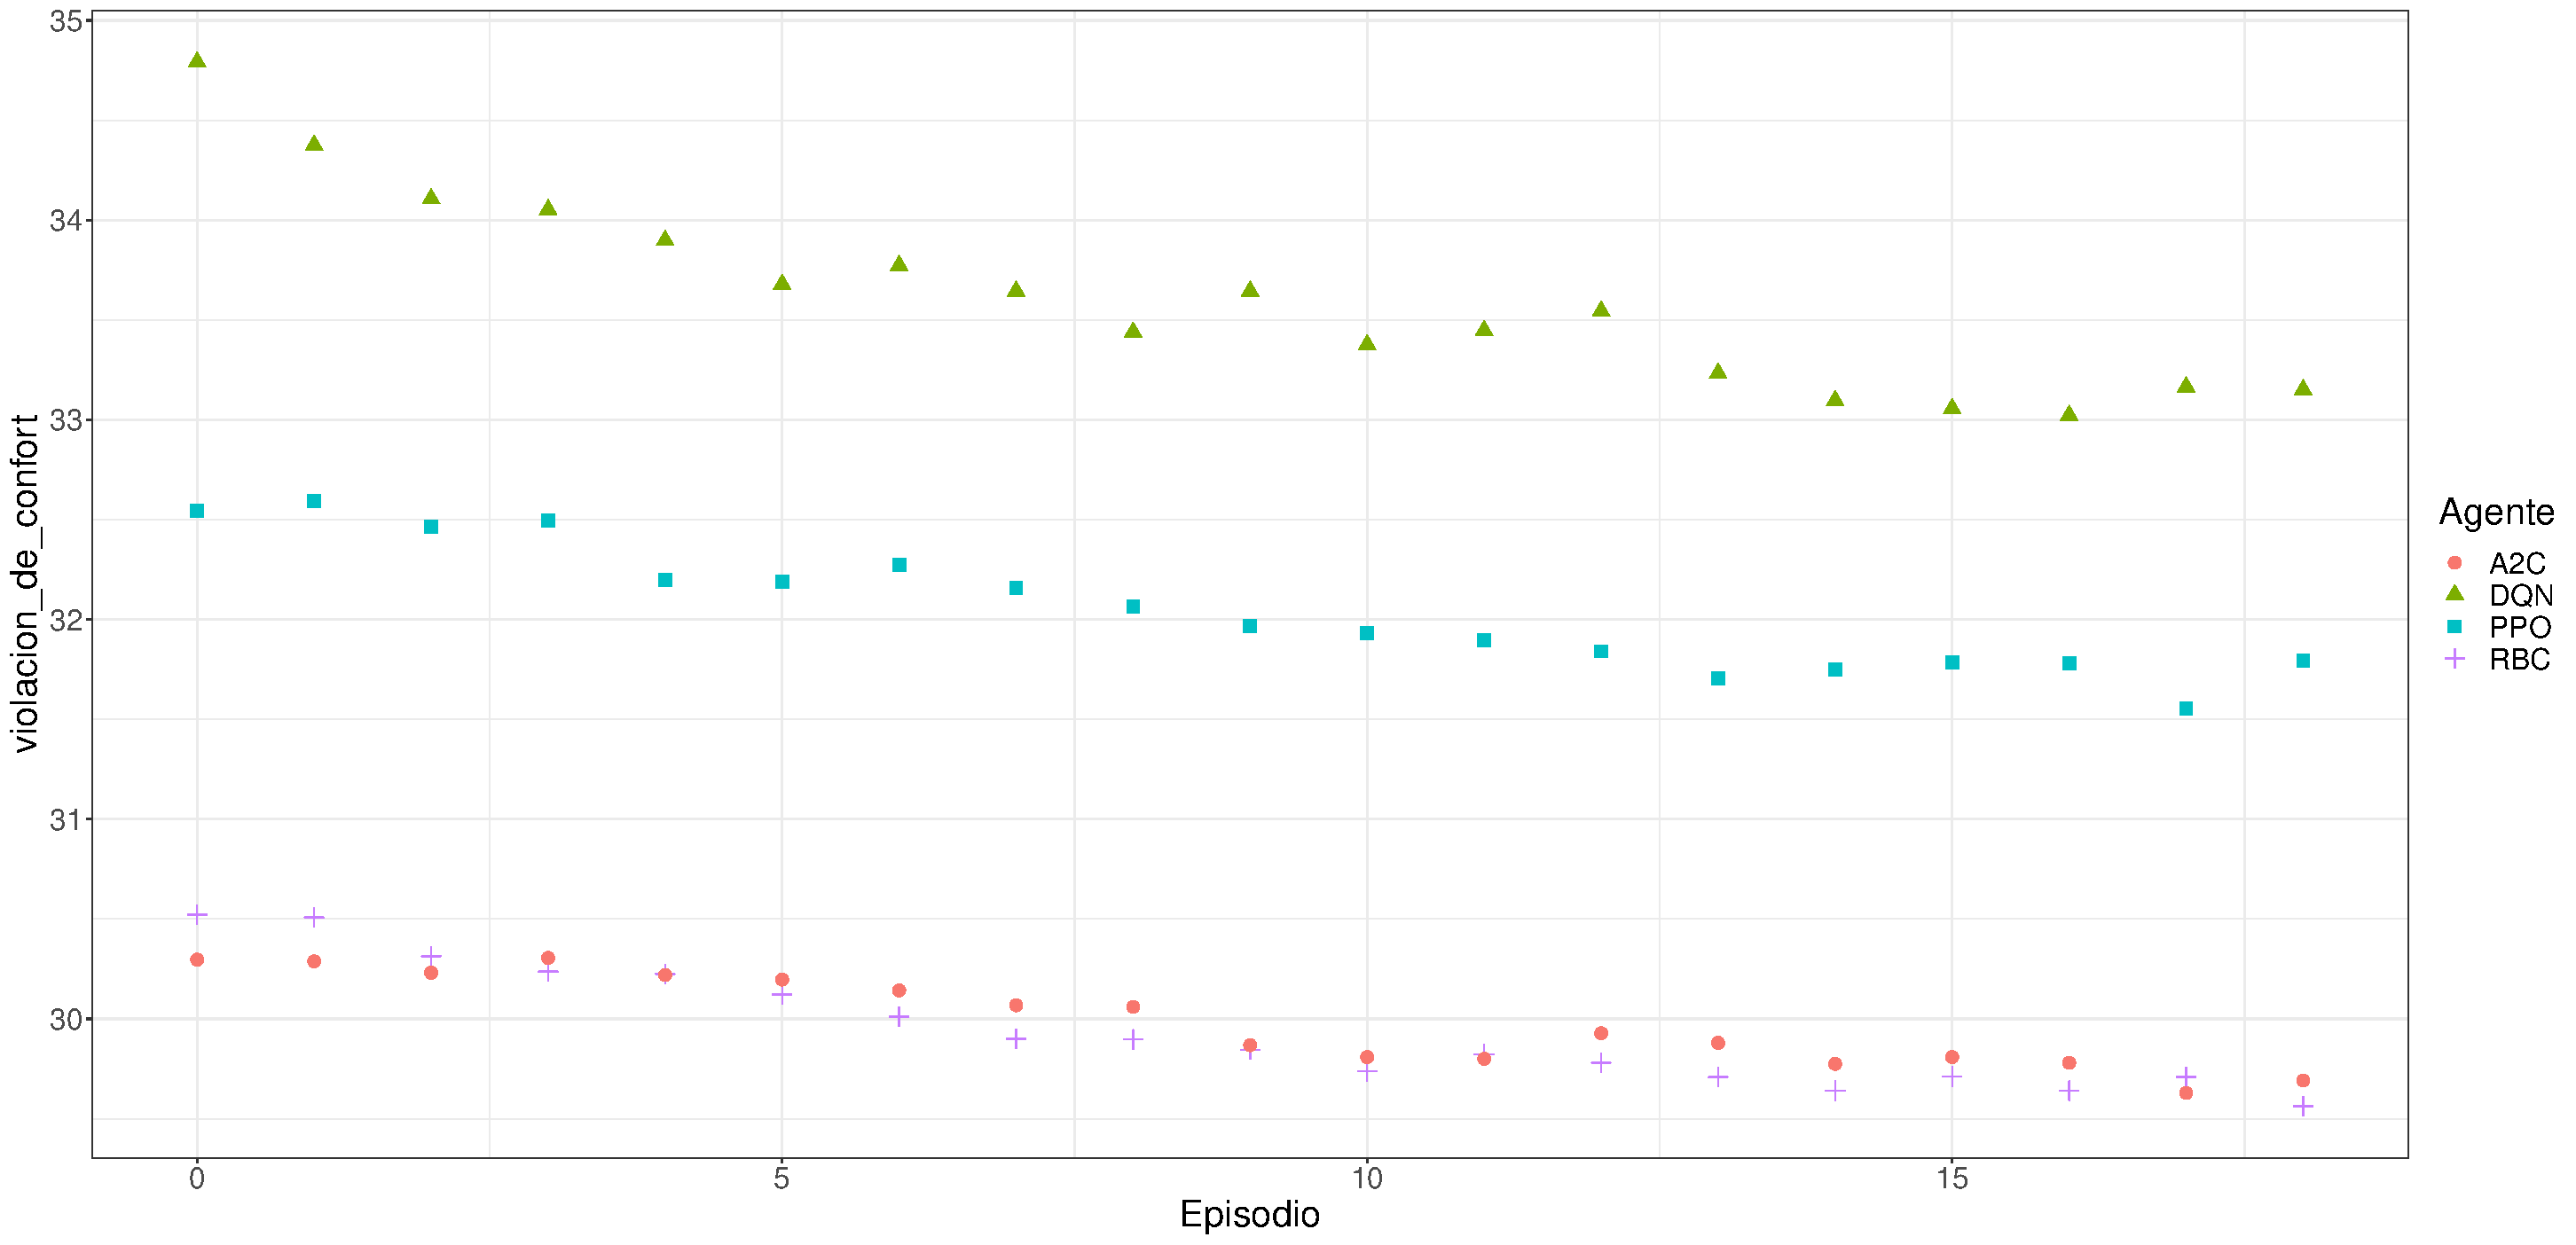
\includegraphics[width=\textwidth]{imagenes/confort-disc-mixed.pdf}
    \caption{Ejemplo de la violación de confort obtenida en la validación de los agentes entrenados en el entorno \textit{discrete-stochastic-mixed}}
    \label{fig:confort-disc-mixed}
\end{figure}

\begin{figure}
    \centering
    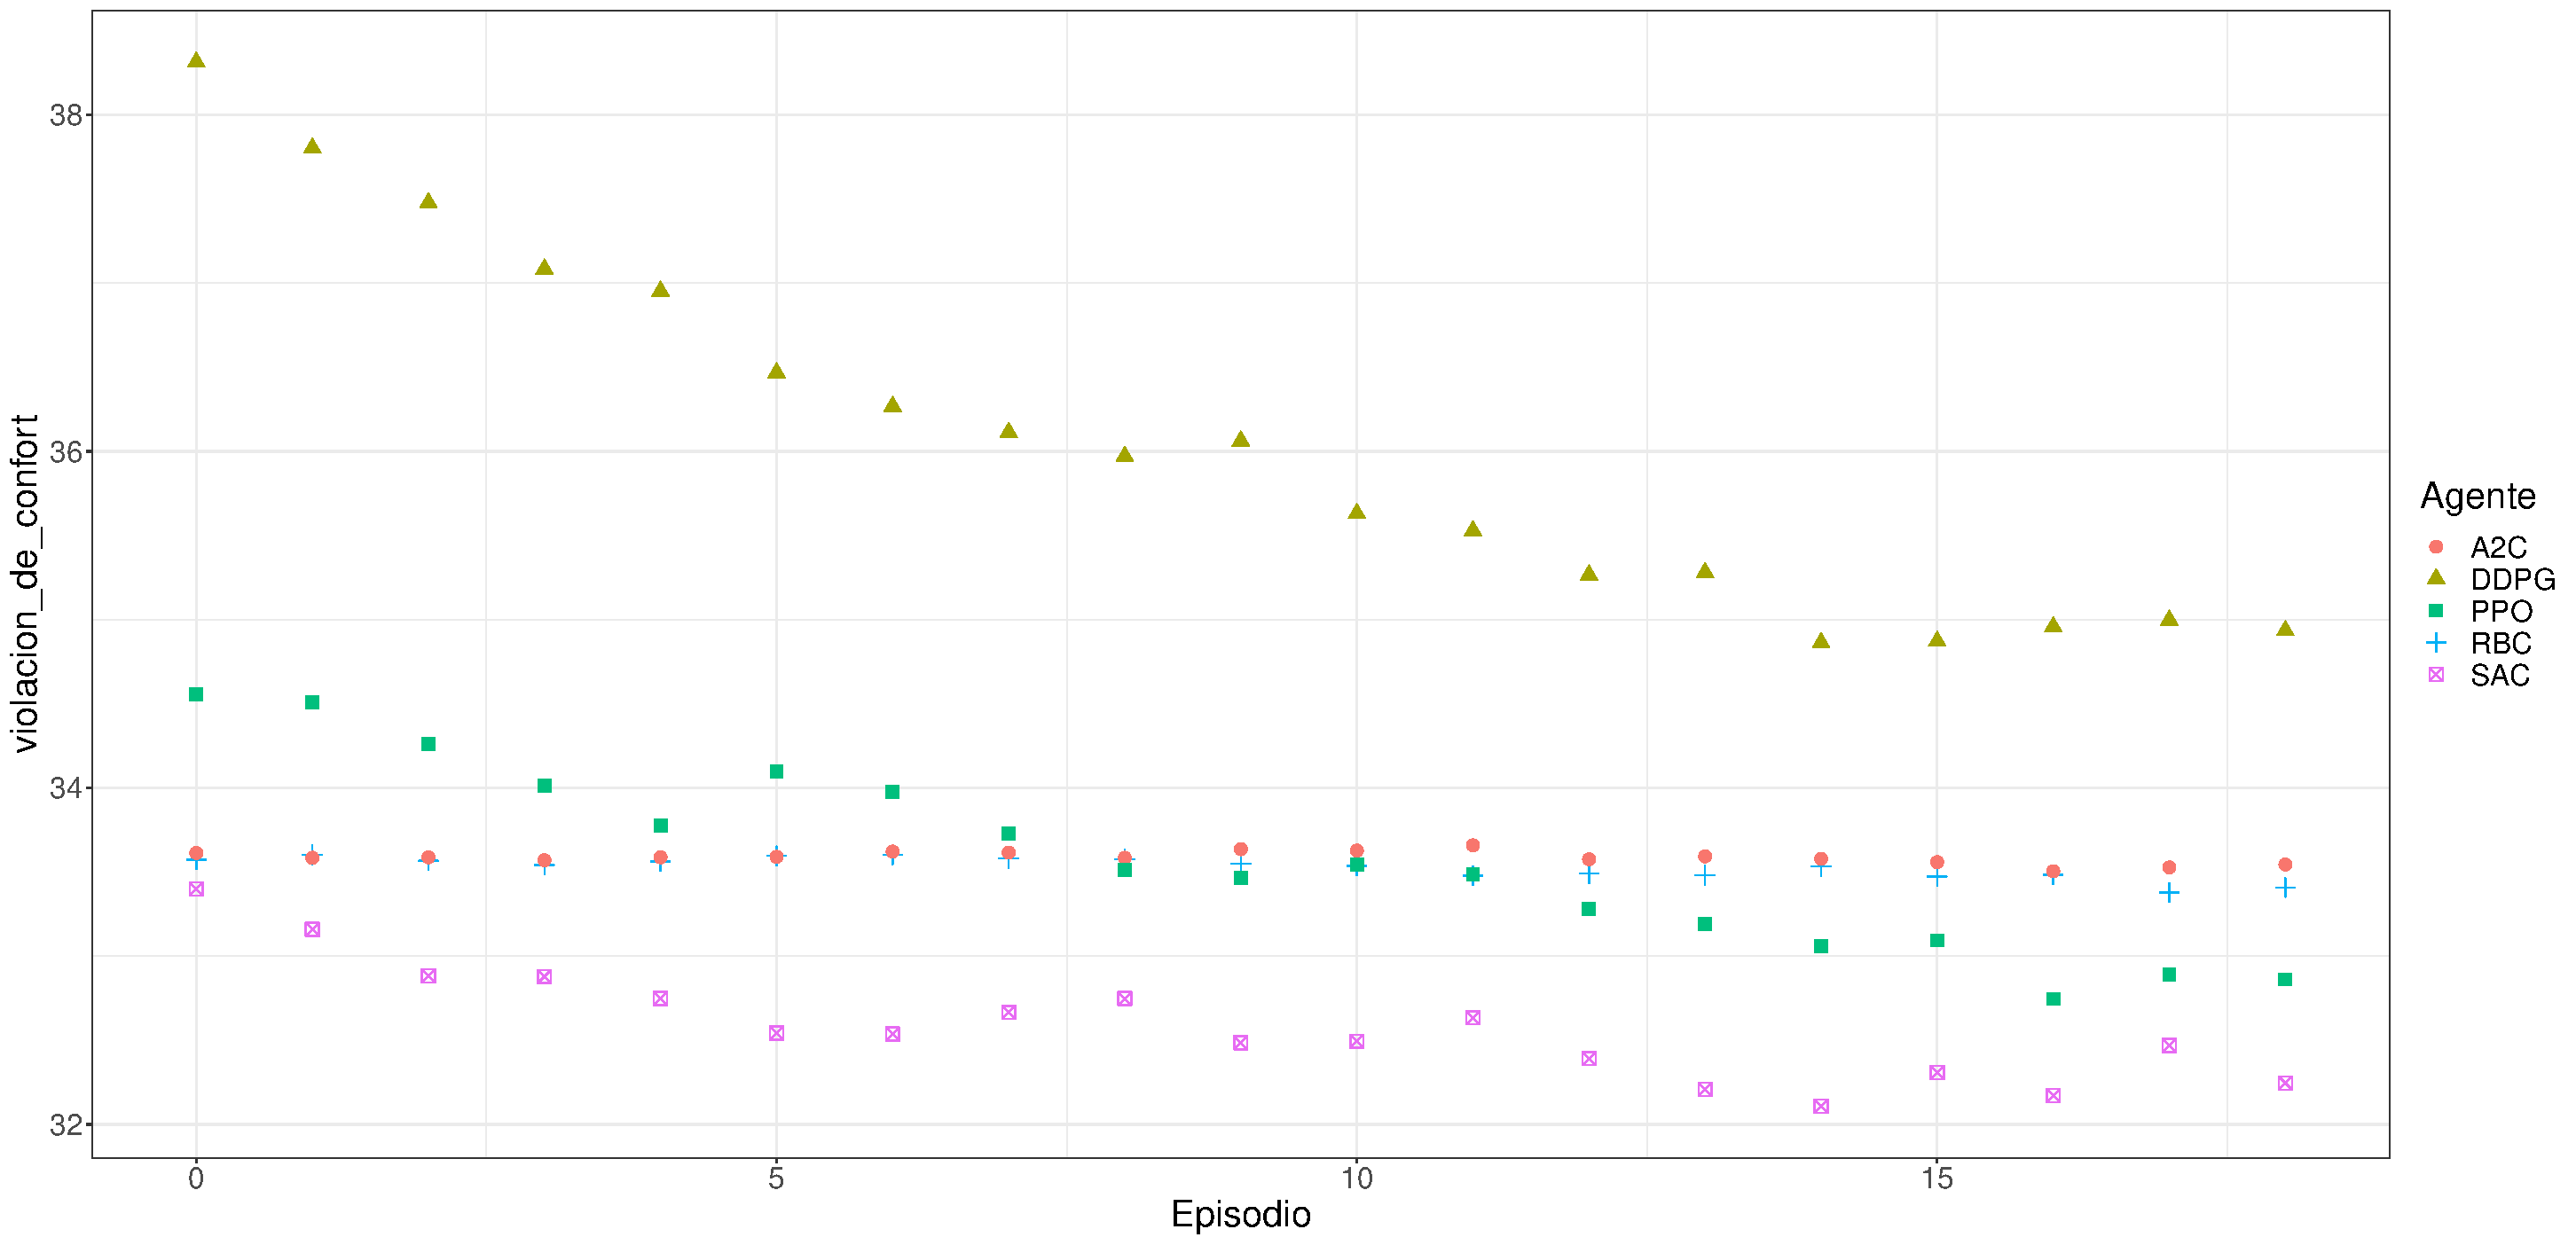
\includegraphics[width=\textwidth]{imagenes/confort-cont-mixed.pdf}
    \caption{Ejemplo de la violación de confort obtenida en la validación de los agentes entrenados en el entorno \textit{continuous-stochastic-mixed}}
    \label{fig:confort-cont-mixed}
\end{figure}

Por último, al igual que en el caso del consumo energético, en las Figuras \ref{fig:confort-disc-mixed} y \ref{fig:confort-cont-mixed} se aprecia cómo los porcentajes de violación de confort empeoran a medida que el clima del entorno cuenta con un mayor ruido acumulado.

\subsubsection{Recompensa}

Finalmente, abordemos el equilibrio entre la minimización del consumo y la maximización del confort, el cual queda reflejado en la función de recompensa empleada. 

En los entornos discretos, A2C y RBC lograron resultados similares, sin apenas variación en sus recompensas medias y superando a las de PPO y DQN en todos los climas (ver Tabla \ref{tb:disc-stats}).

Por otro lado, los resultados más llamativos se dieron en los entornos continuos. En el clima cálido (Figura \ref{fig:recompensa-cont-hot}), las mejoras que SAC y DDPG supusieron frente al RBC fueron del $5.41\%$, mientras que SAC logró superar al RBC en los climas frío y templado con mejoras del $4.73\%$ y $4.71\%$, respectivamente. Estos resultados quedan resumidos en la Tabla \ref{tb:cont-stats}.

En base a estos resultados, se observa que los agentes de DRL en entornos discretos no lograron superar el rendimiento de un RBC. Por el contrario, DDPG y SAC demostraron garantizar un mayor confort y un menor consumo energético que un controlador basado en reglas convencional.

\begin{table}
    \centering
    \caption{Recompensas medias obtenidas por los agentes entrenados en entornos discretos a lo largo de 20 episodios de validación}
    \label{tb:disc-stats}
    \resizebox{0.8\textwidth}{!}{%
    \begin{tabular}{ccccccc}
     & \multicolumn{2}{c}{\textbf{HOT}} & \multicolumn{2}{c}{\textbf{COOL}} & \multicolumn{2}{c}{\textbf{MIXED}} \\ \hline
     & \textit{media} & \textit{desv} & \textit{media} & \textit{desv} & \textit{media} & \textit{desv} \\ \hline
    \textbf{RBC} & \textbf{-.485} & .004 & -.355 & .038 & \textbf{-.422} & .01 \\ \hline
    \textbf{A2C} & -.486 & .005 & \textbf{-.354} & .04 & -.424 & .011 \\ \hline
    \textbf{PPO} & -.502 & .004 & -.394 & .04 & -.436 & .001 \\ \hline
    \textbf{DQN} & -.493 & .004 & -.362 & .038 & -.44 & .008 \\ \hline
    \end{tabular}%
    }
\end{table}

\begin{table}
    \centering
    \caption{Recompensas medias obtenidas por los agentes entrenados en entornos continuos a lo largo de 20 episodios de validación}
    \label{tb:cont-stats}
    \resizebox{0.8\textwidth}{!}{%
    \begin{tabular}{ccccccc}
     & \multicolumn{2}{c}{\textbf{HOT}} & \multicolumn{2}{c}{\textbf{COOL}} & \multicolumn{2}{c}{\textbf{MIXED}} \\ \hline
     & \textit{media} & \textit{desv} & \textit{media} & \textit{desv} & \textit{media} & \textit{desv} \\ \hline
    \textbf{RBC} & -.481 & .003 & -.338 & .036 & -.403 & .013 \\ \hline
    \textbf{A2C} & -.479 & .003 & -.341 & .04 & -.403 & .013 \\ \hline
    \textbf{PPO} & -.496 & .002 & -.351 & .039 & -.403 & .011 \\ \hline
    \textbf{DDPG} & \textbf{-.455} & .002 & -.323 & .041 & -.461 & .004 \\ \hline
    \textbf{SAC} & \textbf{-.455} & .002 & \textbf{-.322} & .042 & \textbf{-.384} & .011 \\ \hline
    \end{tabular}%
    }
\end{table}

\begin{figure}
    \centering
    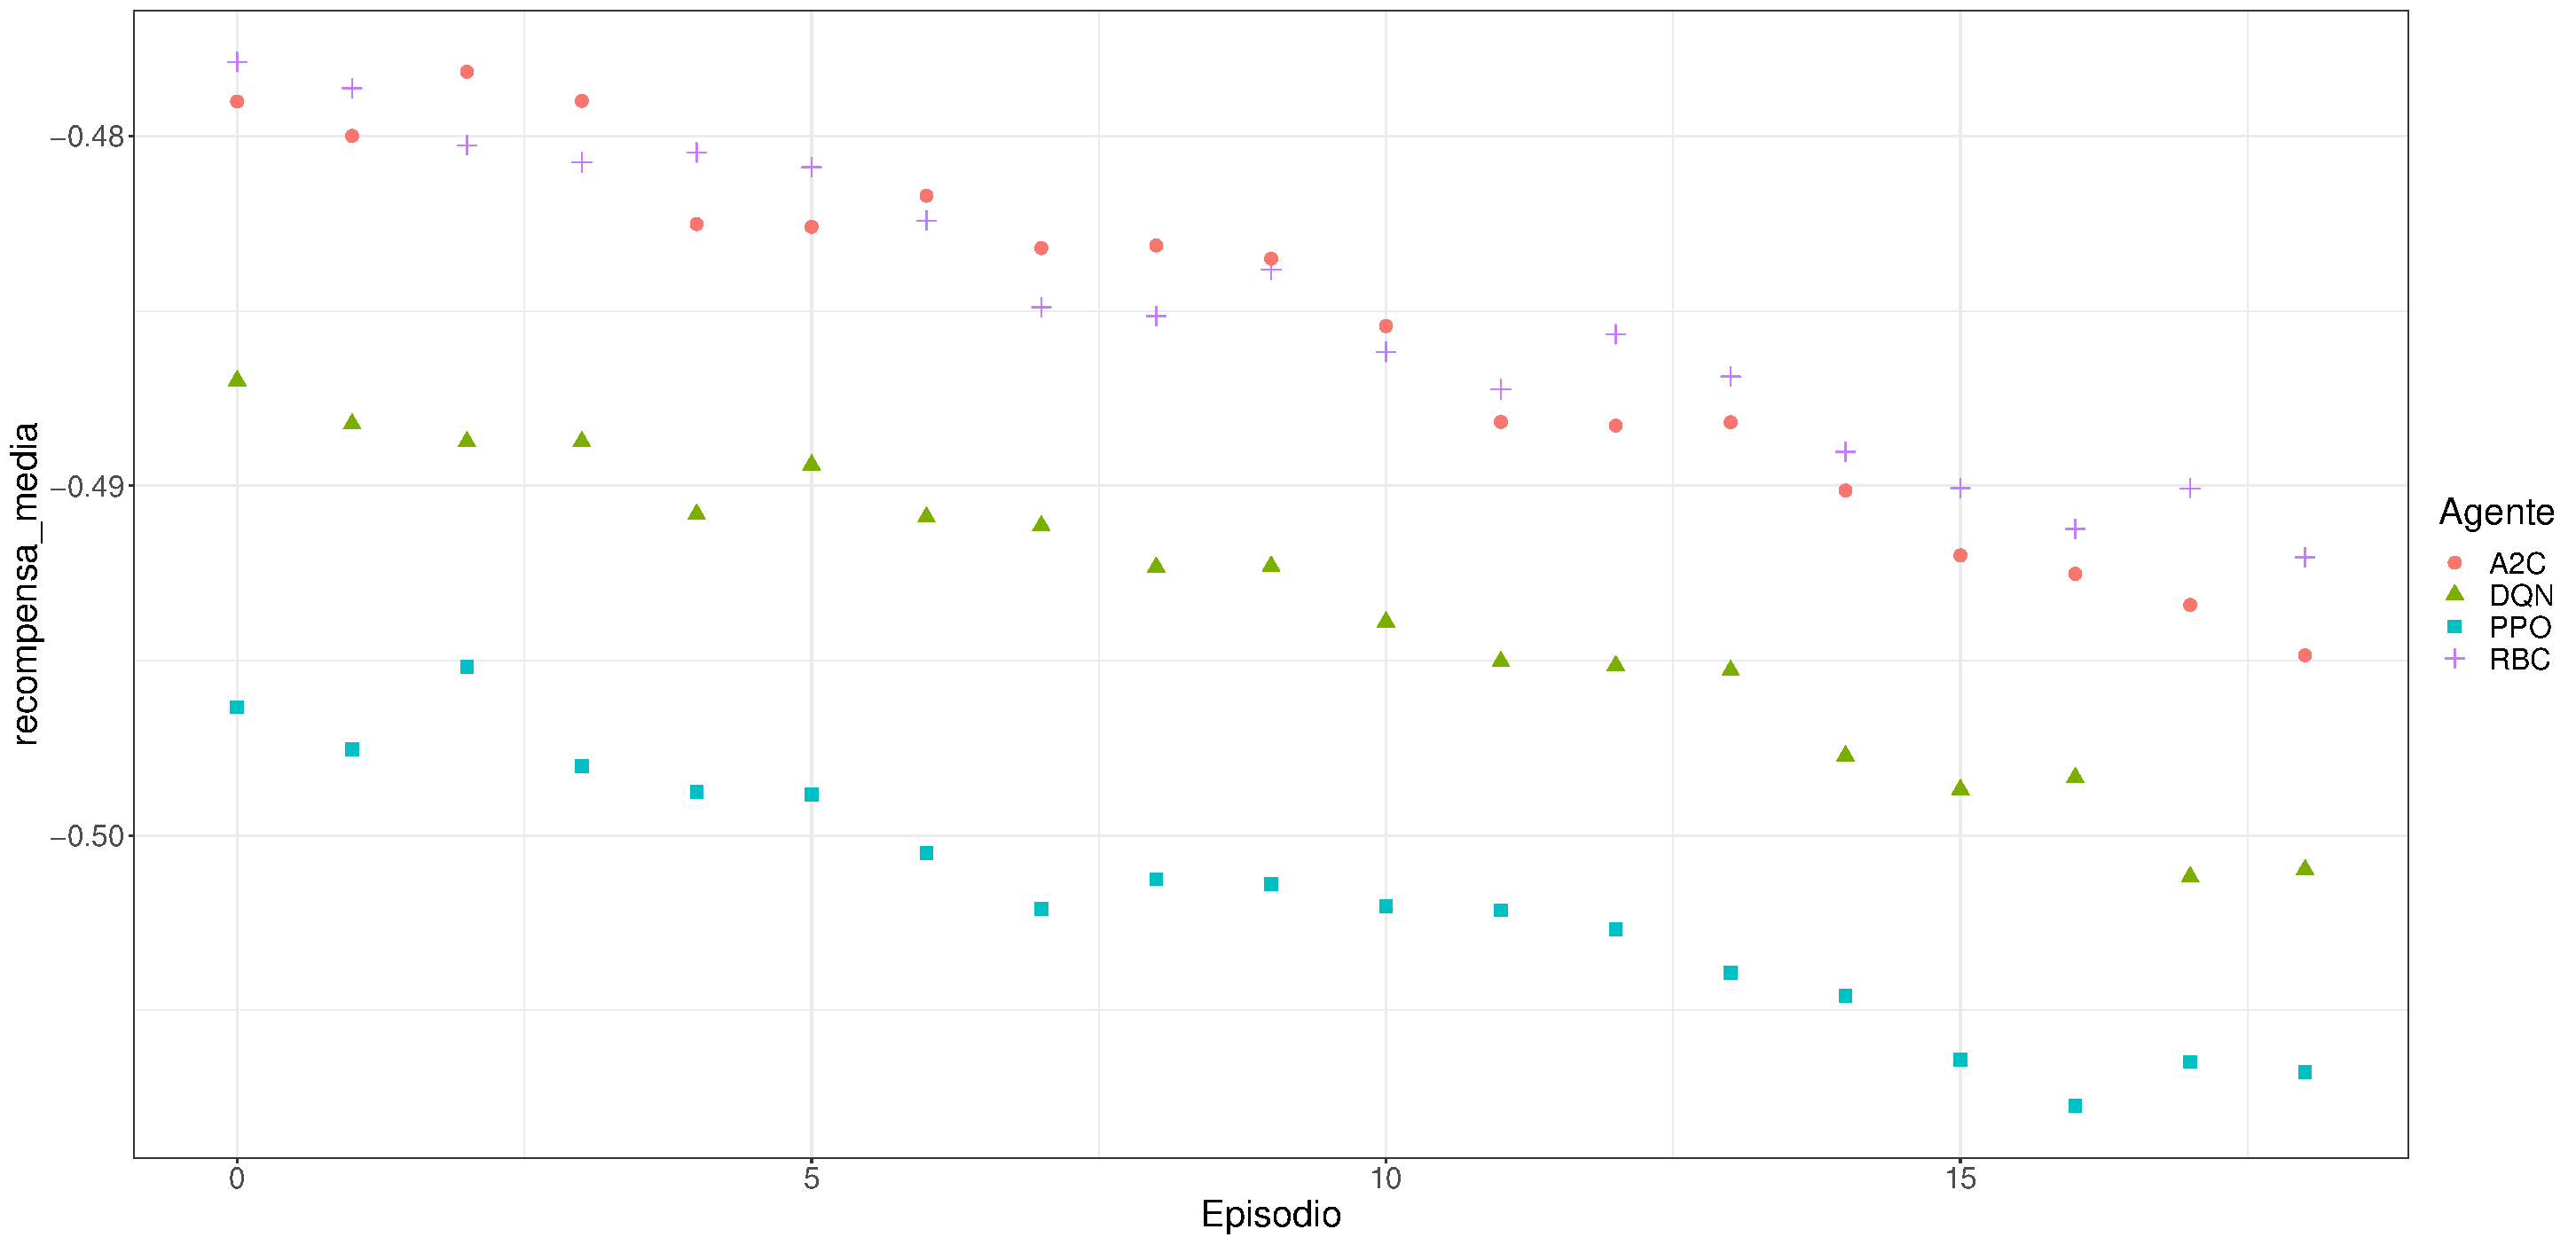
\includegraphics[width=\textwidth]{imagenes/recompensa-disc-hot.pdf}
    \caption{Ejemplo de la recompensa media obtenida en la validación de los agentes entrenados en el entorno \textit{discrete-stochastic-hot}}
    \label{fig:recompensa-disc-hot}
\end{figure}

\begin{figure}
    \centering
    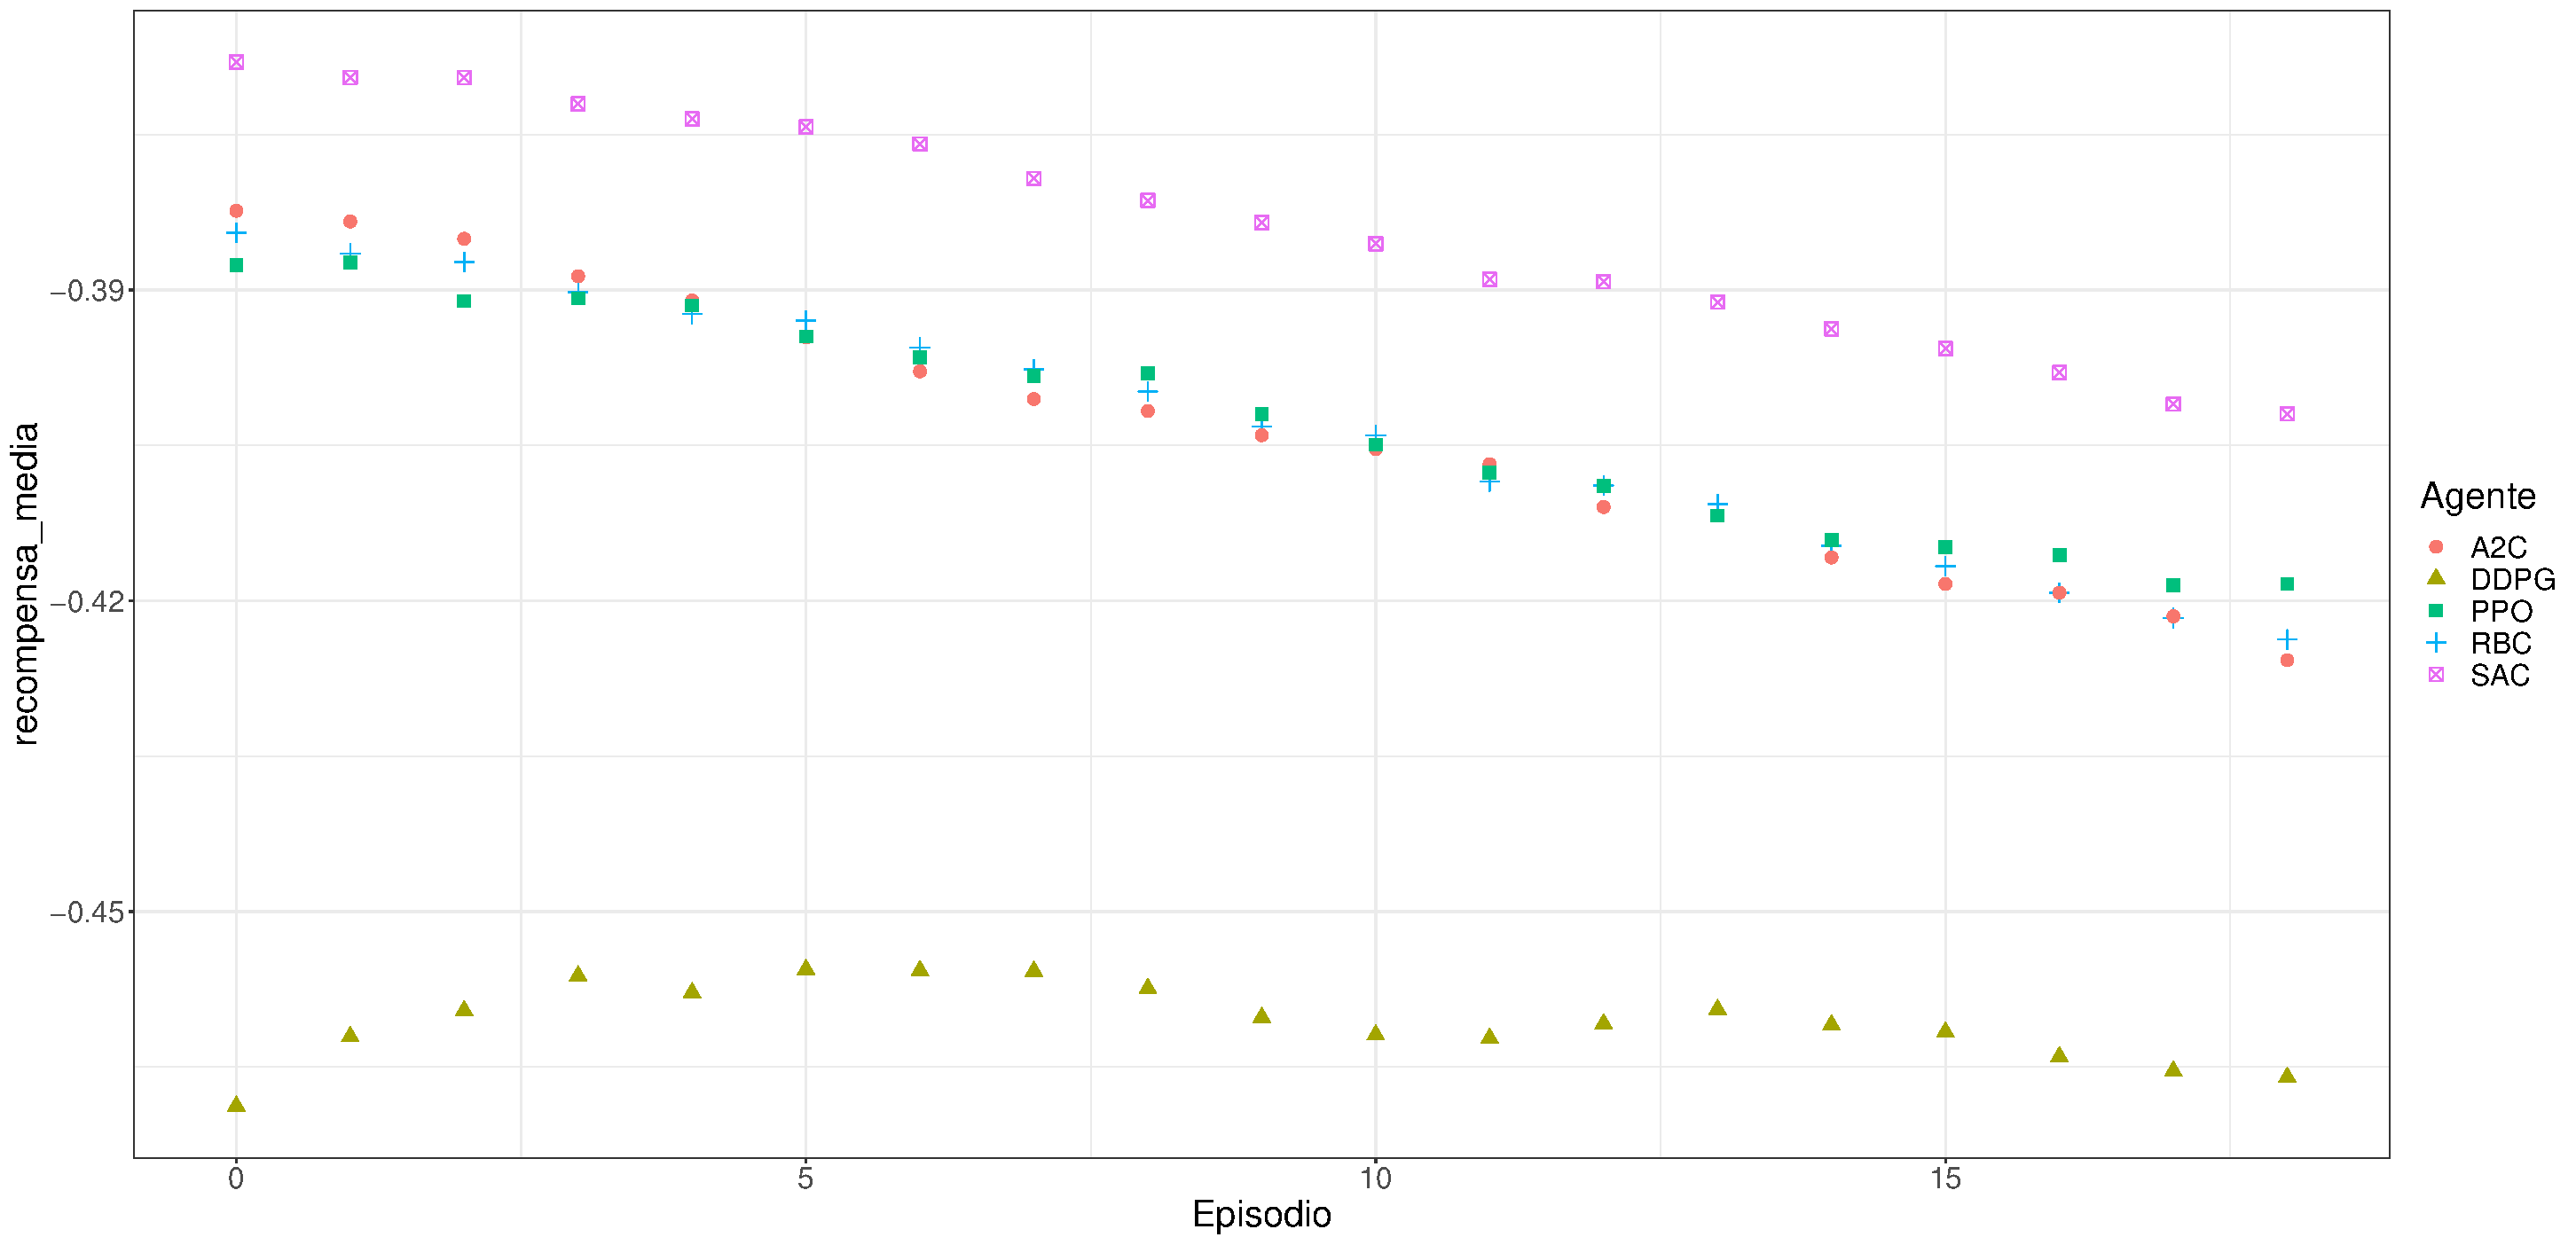
\includegraphics[width=\textwidth]{imagenes/recompensa-cont-hot.pdf}
    \caption{Ejemplo de la recompensa media obtenida en la validación de los agentes entrenados en el entorno \textit{continuous-stochastic-hot}}
    \label{fig:recompensa-cont-hot}
\end{figure}

\section{Experimentación avanzada}

Una vez estudiado el desempeño de los agentes en cada tipo de entorno, se llevaron a cabo una serie de experimentos adicionales destinados a comprender en profundidad otros aspectos del problema en cuestión. Dichos experimentos fueron realizados empleando el agente basado en DDPG, al tratarse de uno de los algoritmos que mejores resultados proporcionó en la mayoría de entornos y métricas de evaluación. El hecho de emplear DDPG frente a SAC se debió a que DDPG requirió menores tiempos de entrenamiento.

En las siguientes subsecciones se detallarán dichos experimentos y los resultados obtenidos.

\subsection{Equilibrio confort-consumo}
\label{sec:conf-con}

Como ya se estudió en la sección \ref{sec:formulacion}, el control HVAC por medio de RL supone el empleo de una función de recompensa que contemple tanto la maximización del confort como la reducción del consumo energético. Así, el objetivo a perseguir será la búsqueda del equilibrio entre ambas partes de la recompensa.

En la formulación del problema también abordamos cómo cada una de estas partes cuenta con una ponderación: $w_t$ y $(1-w_t)$; estos pesos nos permiten definir la importancia asignada al confort y al consumo, respectivamente, o lo que es lo mismo: su influencia en la función de recompensa.

Si atendemos a los experimentos llevados a cabo en la sección \ref{sec:evaluacion-agentes}, la importancia asignada a cada parte de la recompensa fue la misma, con $w_t=0.5$. De forma ilustrativa, pasemos ahora a asignar una mayor importancia al \textbf{consumo} y comparar los resultados obtenidos. Para llevar a cabo esta experimentación, emplearemos el agente basado en DDPG, en un clima templado y un espacio de acciones continuo.

Como se muestra en la Figura \ref{fig:pesos-consumo}, abogar por un 75\% de peso para el consumo (y, por tanto, un 25\% para el confort) frente a una ponderación equilibrada (50\%-50\%) supone:

\begin{itemize}
    \item Un menor consumo energético medio, ya que este toma una mayor importancia en la función de recompensa. Esto se observa especialmente bien si atendemos a la penalización por consumo, mucho menor para una ponderación 75\%-25\%.
    \item Un aumento de casi el 50\% de la violación del confort, debido a que el agente centra sus esfuerzos en reducir el consumo a toda costa. De nuevo, la penalización por confort es considerablemente mayor para el caso 75\%-25\%.
\end{itemize}

\begin{figure}
    \centering
    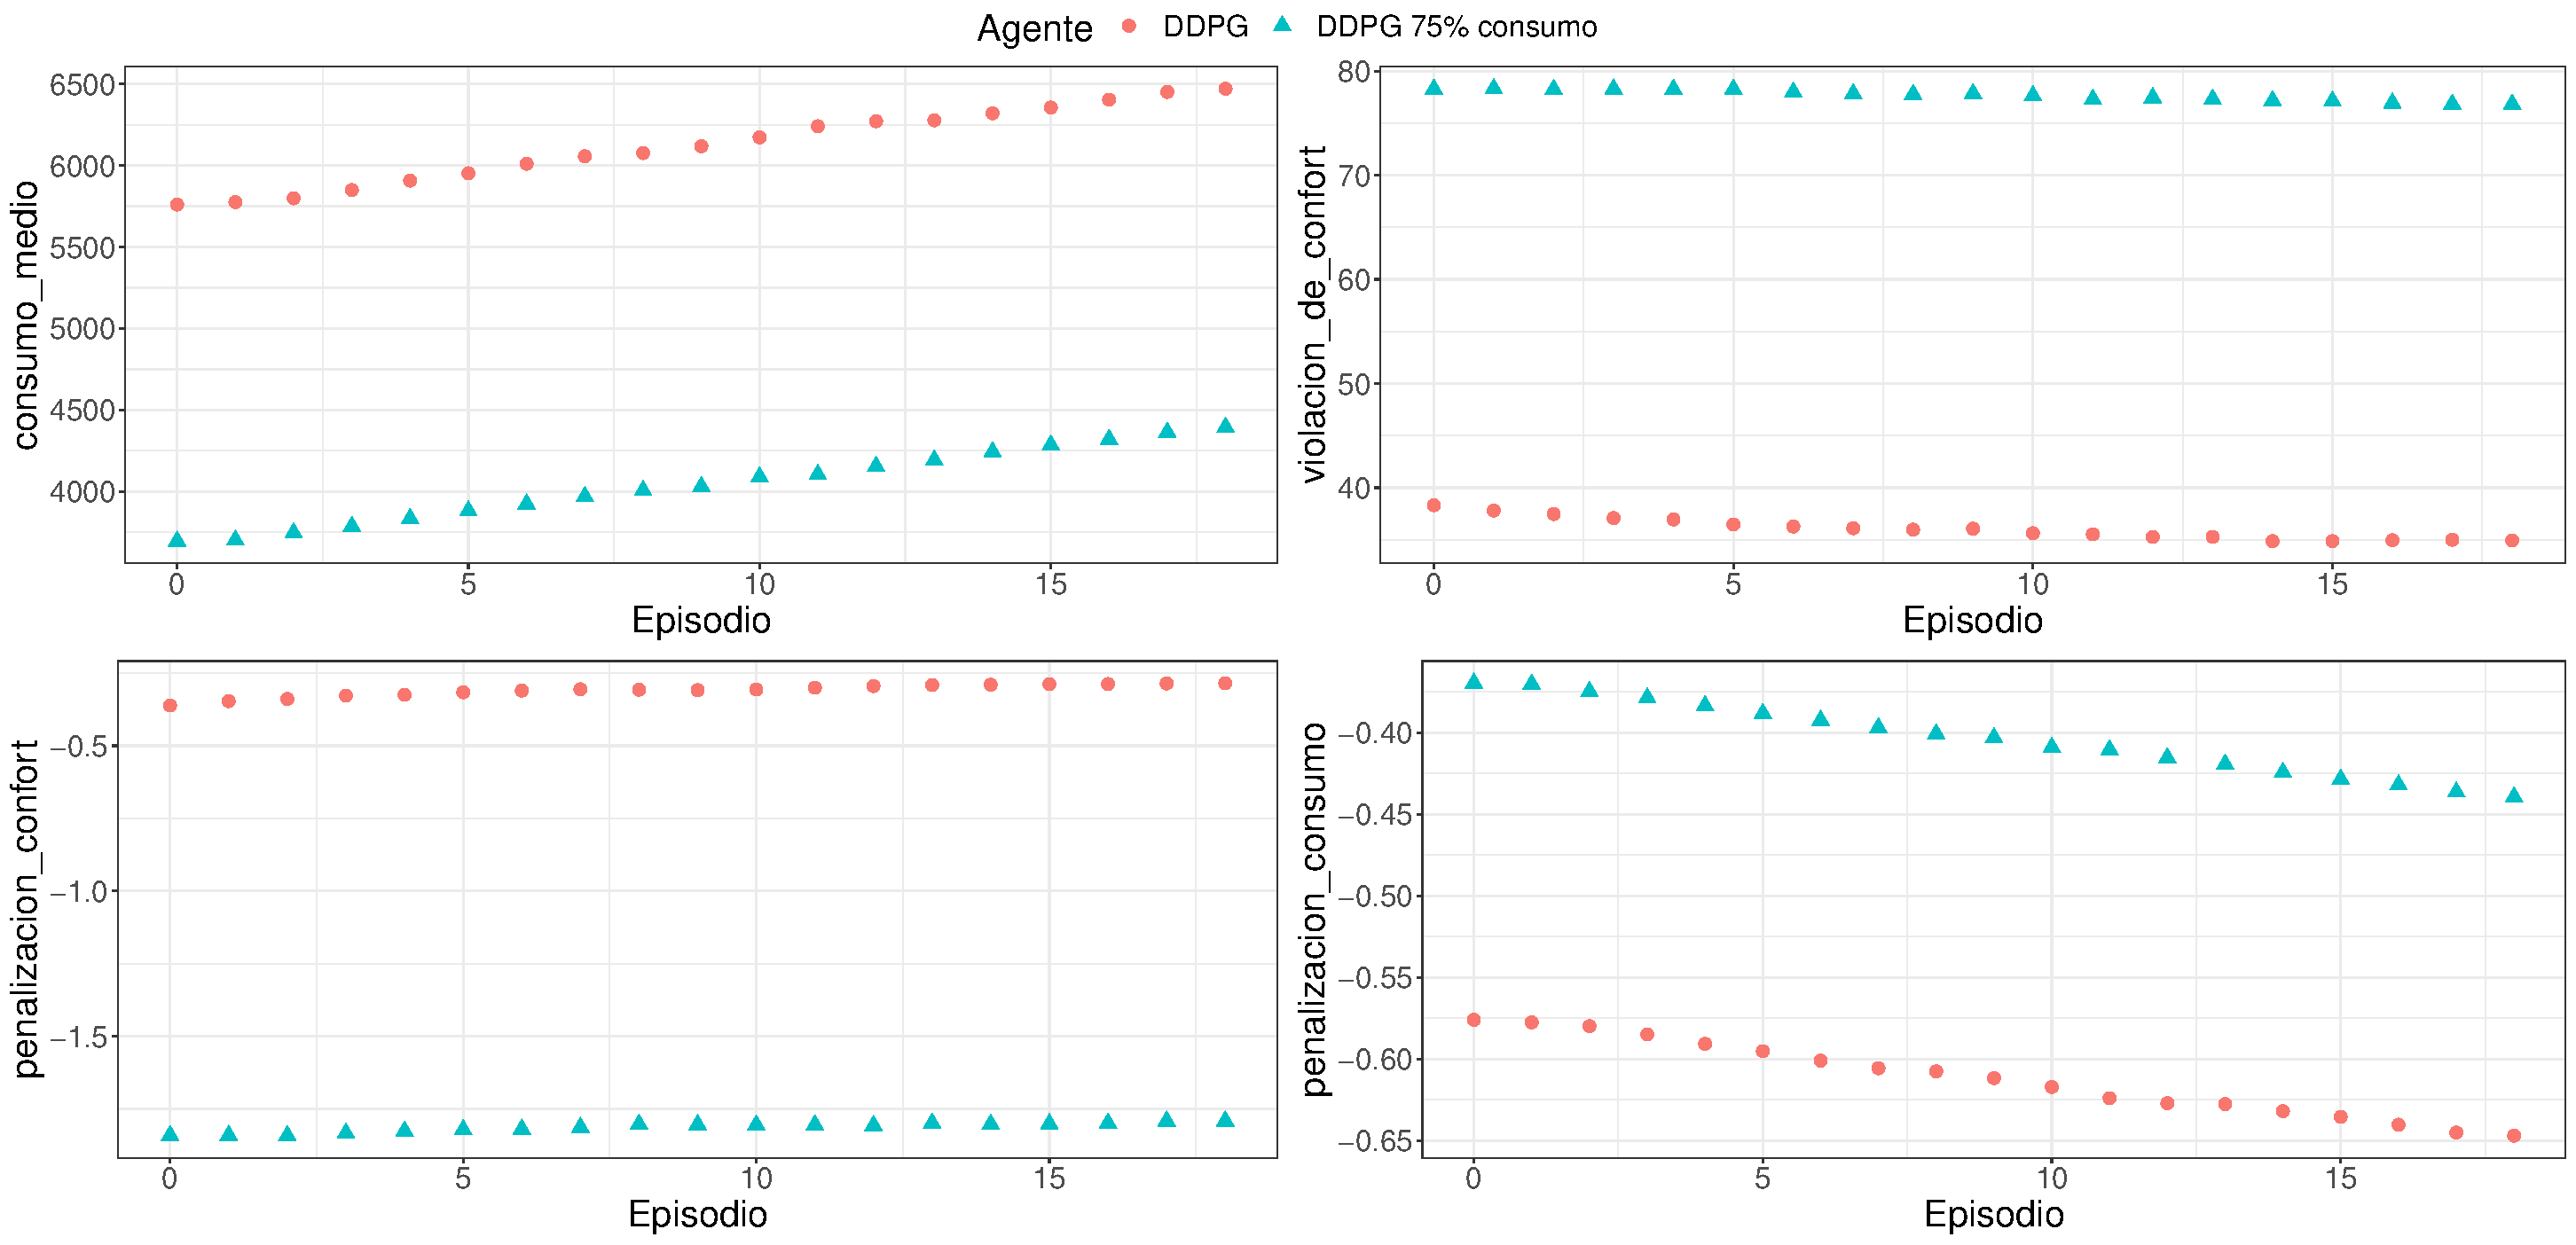
\includegraphics[width=\textwidth]{imagenes/energy-weights-DDPG.pdf}
    \caption{Resultados tras la validación de un agente entrenado con DDPG para diferentes ponderaciones de consumo}
    \label{fig:pesos-consumo}
\end{figure}

Con este ejemplo se ha tratado de ilustrar la flexibilidad que Energym nos ofrece a la hora de comparar diferentes ponderaciones de confort y consumo. Dichos pesos son un parámetro más a definir por el usuario, permitiendo una mayor personalización de los entornos y dotando a Energym de nuevas capacidades de experimentación. 

En conclusión, el equilibrio confort-consumo personalizable en Energym abre un amplio abanico de posibilidades, mayor aún si consideramos ponderaciones dinámicas o funciones de recompensa más complejas, fácilmente definibles a partir de los \textit{wrappers} ofrecidos por OpenAI Gym.

\subsection{Pruebas de robustez}
\label{sec:robustez}

Pasemos a estudiar la eficiencia de los agentes en entornos para los cuales no han sido entrenados. Estas ``pruebas de robustez'' nos permiten saber hasta qué punto un agente es capaz de generalizar y obtener un buen rendimiento en condiciones no experimentadas durante su entrenamiento.

Así, el experimento planteado consistirá en la evaluación de un agente entrenado en un clima \textbf{templado} en los entornos \textbf{cálido} y \textbf{frío}. Esto nos permitirá conocer la versatilidad de un agente entrenado en un clima con temperaturas más extremas.

Veamos, pues, los resultados obtenidos para cada prueba de robustez. De nuevo, utilizaremos el agente basado en DDPG en las mismas condiciones que la experimentación anterior.

Como podemos ver en la Figura \ref{fig:recompensa-robustez}, en un período de 20 episodios un agente entrenado en un clima templado ofrece un mejor control en un clima cálido que en uno mixto. Esto puede deberse a que el clima mixto supone una complejidad superior, al contar con un mayor rango de temperaturas a cubrir. No ocurre lo mismo para el agente entrenado en un entorno mixto y probado en uno frío. En comparación con el caso anterior, el bajo rendimiento podría deberse a que un clima templado es más próximo a las características del cálido que del frío, o bien que el clima frío requiera, por lo general, un mayor consumo energético.

\begin{figure}
    \centering
    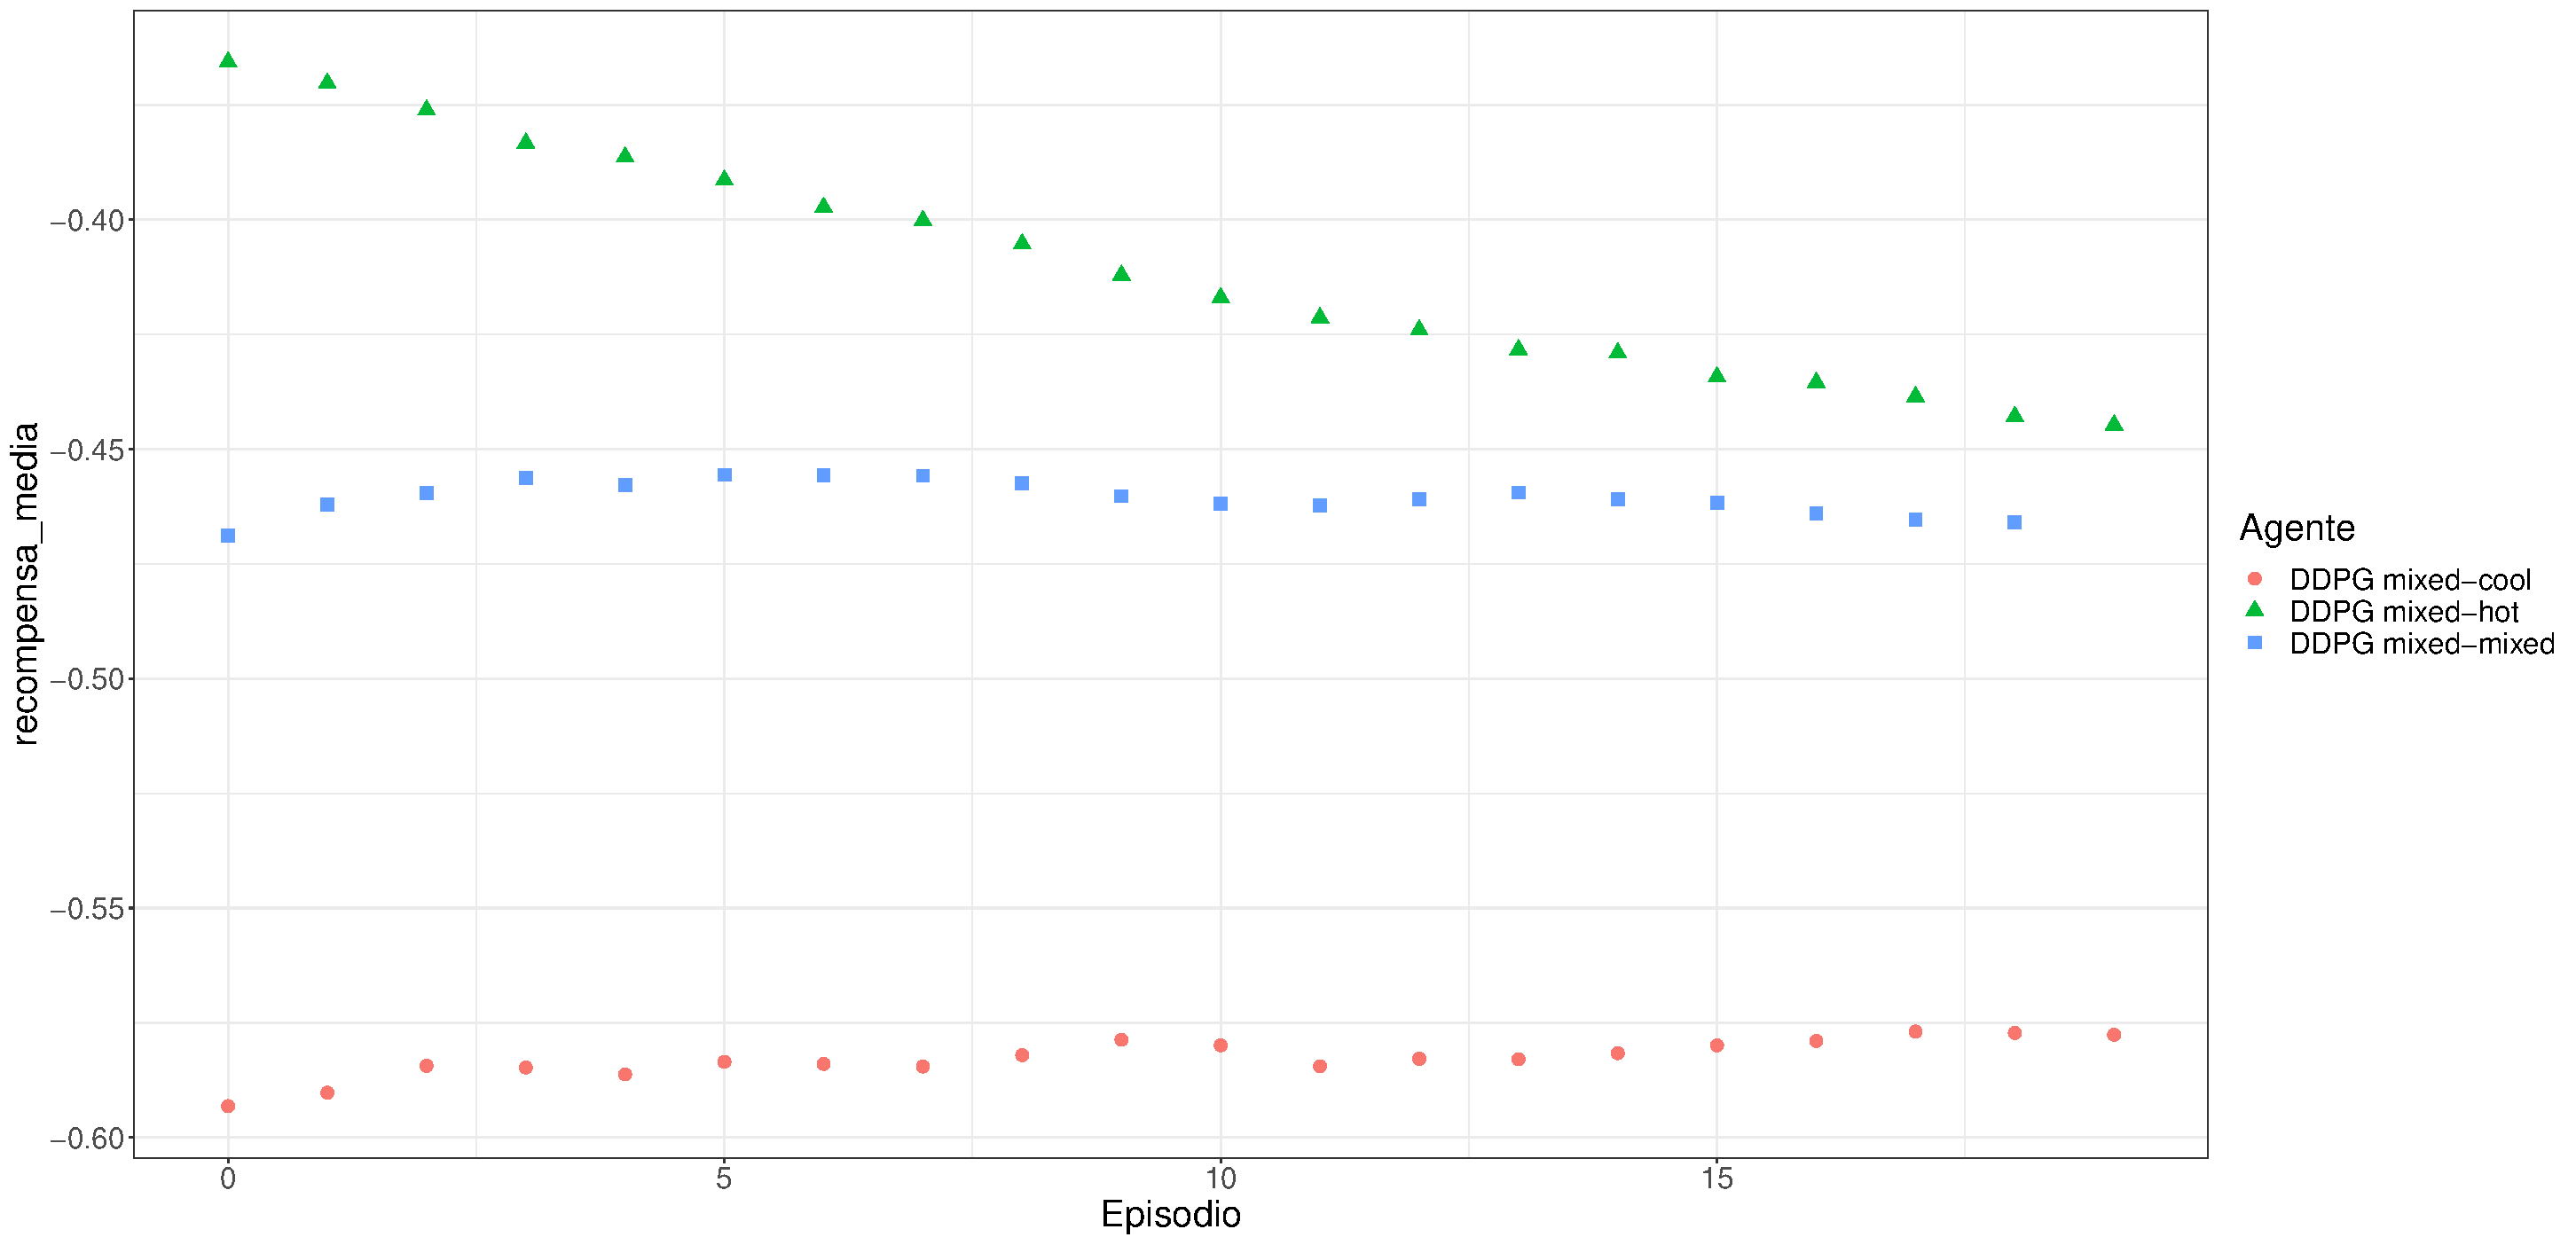
\includegraphics[width=\textwidth]{imagenes/recompensa-robustez.pdf}
    \caption{Evaluación del agente entrenado en clima \textit{mixed} y ejecutado en \textit{mixed}, \textit{cool} y \textit{hot}}
    \label{fig:recompensa-robustez}
\end{figure}

Este tipo de pruebas nos permiten conocer si el entrenamiento de un agente en un determinado tipo de entorno podría ser prescindible. Por ejemplo, en este caso, podríamos emplear el agente \textit{mixed} en el entorno \textit{hot} y obtendríamos mejores resultados, lo que reduce nuestro interés por entrenar un agente para cada entorno, pudiendo disponer de un único agente que opere bien en múltiples contextos.

A modo de reflexión, una discusión más profunda sobre los resultados ofrecidos por este tipo de experimentos sería un interesante debate a abordar de la mano de una persona experta en este campo. Aunque dicha discusión escapa de los objetivos de este proyecto, en esta sección hemos visto cómo Energym podría ser utilizado para un estudio en profundidad ante este tipo de situaciones.

\subsection{\textit{Curriculum learning}}
\label{sec:cv-learning}

En esta última sección abordaremos la aplicación de \textit{curriculum learning} en nuestro problema. Se trata de un tipo de aprendizaje progresivo, consistente en partir del entrenamiento en escenarios sencillos e ir utilizando el conocimiento adquirido hasta el momento para entrenarse en entornos más complejos.

Este método de aprendizaje ha demostrado ser de gran utilidad, logrando importantes avances en el ámbito del aprendizaje por refuerzo \cite{portelas2020automatic}. Se trata de un tipo de aprendizaje inspirado profundamente en cómo los humanos aprendemos, ya que nuestra formación se basa en un currículo de situaciones de aprendizaje interdependientes de diversa y progresiva complejidad \cite{narvekar2020curriculum}.

En el ámbito de nuestro problema, el aspecto fundamental que marca la complejidad de un entorno es la variabilidad de su clima: es mucho más fácil optimizar el control HVAC en un entorno donde las temperaturas apenas varían a lo largo del año, que en otro donde el clima es más inestable. Así, probaremos a comparar el rendimiento de un agente entrenado directamente sobre un clima \textit{mixed} con otro entrenado en los climas \textit{hot} y \textit{cool}. Utilizaremos DDPG bajo las mismas configuraciones descritas en los experimentos anteriores, siguiendo el proceso de aprendizaje detallado en la Figura \ref{fig:cv-learning}.

\begin{figure}
    \centering
    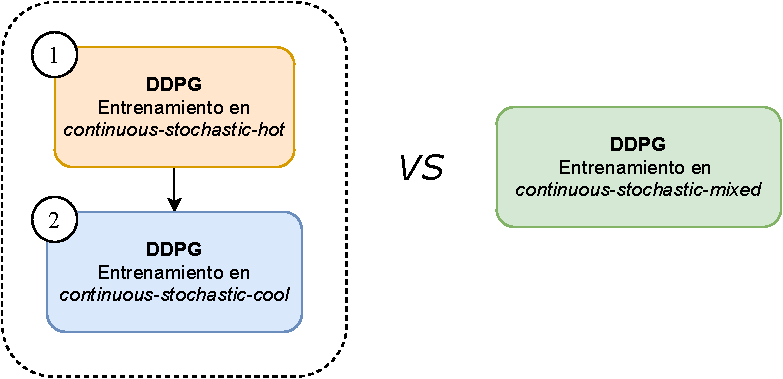
\includegraphics[width=\textwidth]{imagenes/cv-learning.pdf}
    \caption{Experimentación mediante \textit{curriculum learning}}
    \label{fig:cv-learning}
\end{figure}

Una vez realizado el experimento, si atendemos a la Figura \ref{fig:cv-learning-recompensa}  y la Tabla \ref{tb:cv-learning}, observamos que el agente entrenado en un entorno cálido y, posteriormente, en un entorno frío, es capaz de ofrecer mejores resultados que un agente entrenado en un entorno templado. Una posible explicación podría ser que el agente entrenado mediante \textit{curriculum learning} cuenta con una mayor especialización en temperaturas altas y bajas, en contraposición con el agente entrenado en \textit{mixed}, el cual no es capaz de gestionar temperaturas moderadamente fuera de su rango habitual.

\begin{figure}
    \centering
    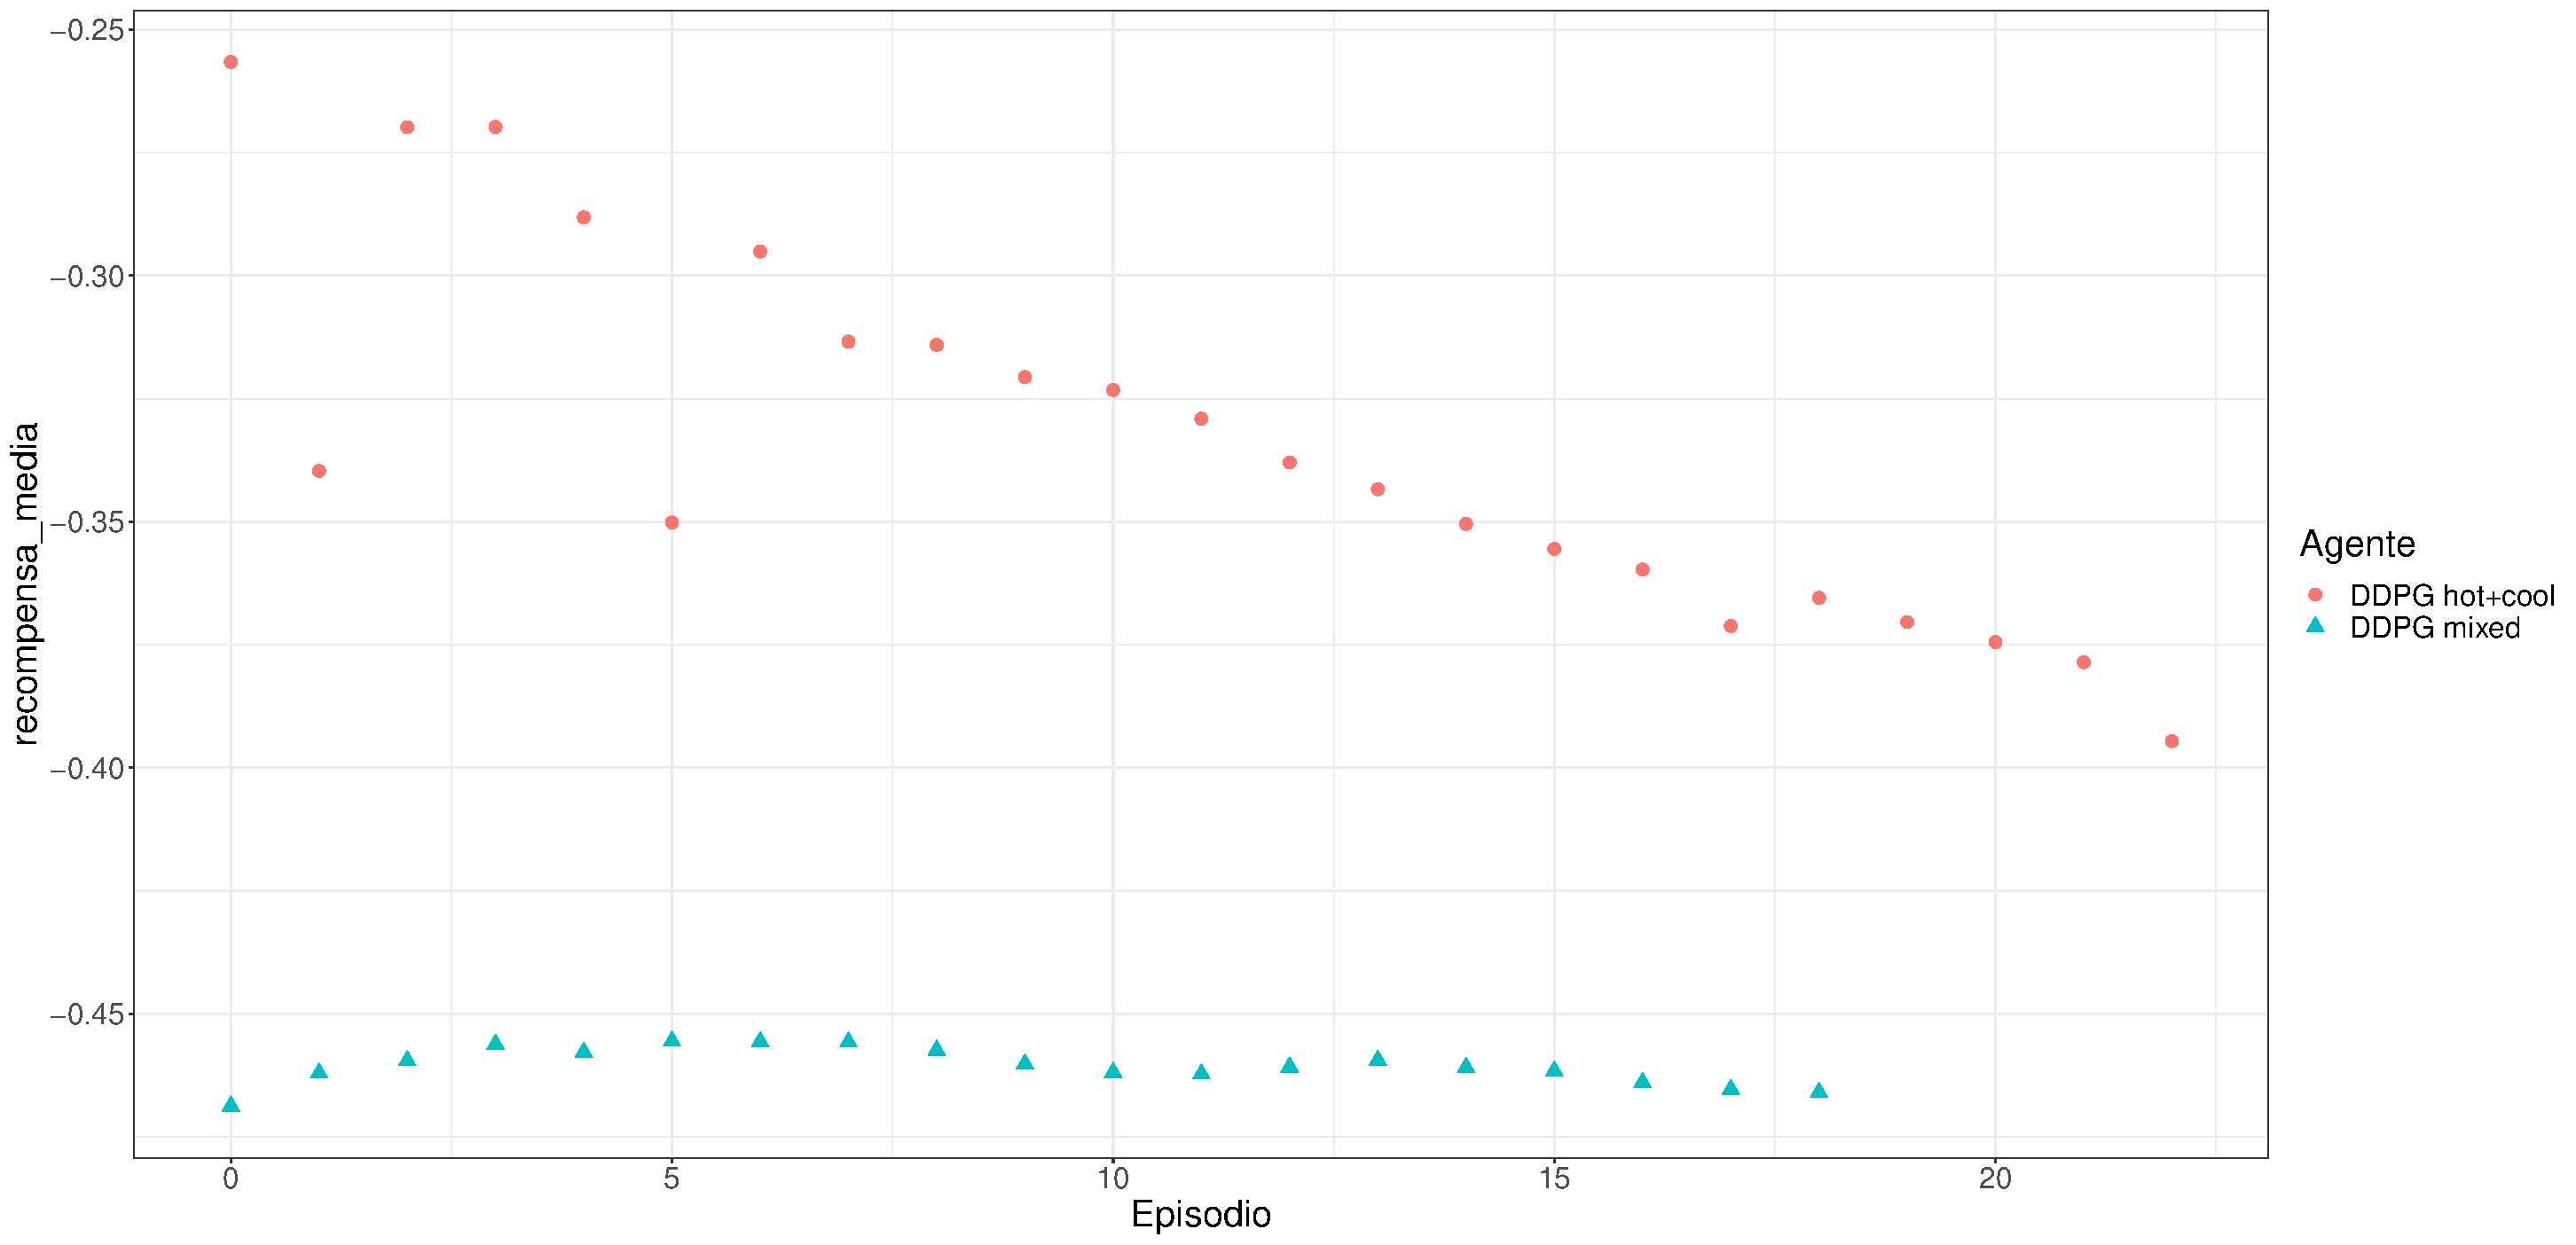
\includegraphics[width=\textwidth]{imagenes/recompensa-cv-learning.pdf}
    \caption{Recompensas medias obtenidas en la experimentación con \textit{curriculum learning}}
    \label{fig:cv-learning-recompensa}
\end{figure}

\begin{table}
    \centering
    \caption{Resultados obtenidos en la validación de DDPG entrenado en \textit{mixed} y DDPG entrenado en \textit{hot} y \textit{cool} sobre el entorno \textit{continuous-mixed}}
    \label{tb:cv-learning}
    \resizebox{\textwidth}{!}{%
    \begin{tabular}{ccccccc}
    \textbf{} & \multicolumn{2}{c}{\textbf{Recompensa}} & \multicolumn{2}{c}{\textbf{Consumo}} & \multicolumn{2}{c}{\textbf{Viol. confort}} \\ \hline
     & \textit{media} & \textit{desv} & \textit{media} & \textit{desv} & \textit{media} & \textit{desv} \\ \hline
    \textbf{DDPG mixed} & -.461 & .004 & 6118.94 & 234.366 & 36.044 & 1.063 \\ \hline
    \textbf{DDPG hot+cool} & \textbf{-.334} & .038 & \textbf{4396.529} & 542.063 & \textbf{34.683} & 2.81 \\ \hline
    \end{tabular}%
    }
\end{table}

Finalmente, se reitera en la idea de que la profundización en estos resultados podrían dar lugar a un amplio debate que va más allá de los objetivos de este trabajo. Así, el principal objetivo de esta sección ha sido demostrar cómo Energym puede ajustarse a un tipo de experimentaciones de mayor complejidad que se alejan de las pruebas convencionales, y que, sin duda alguna, cuentan con un enorme potencial en este campo.
